% Figures for Multi-Scale Oscillatory Analysis of Consumer-Grade Wearable Sensors
% This file contains all figure inclusions for the actigraphy publication

% Figure 1: Multi-Scale Oscillatory Activity Framework
% Position: Section 2 (Theoretical Framework) - After equation (2.1)
% Reason: Establishes the theoretical foundation by showing the 11-scale hierarchical architecture
\begin{figure}[H]
\centering

\includegraphics[width=0.9\textwidth]{figures/multiscale-oscillatory-activity.pdf}
\caption{\textbf{Multi-Scale Oscillatory Activity Framework.} Hierarchical representation of the 11-scale oscillatory system governing human activity patterns. The framework spans from atmospheric gas oscillations ($10^{-7}$--$10^{-4}$~Hz) to quantum membrane dynamics ($10^{12}$--$10^{15}$~Hz), with each scale exhibiting characteristic frequency ranges and coupling mechanisms. Arrows indicate inter-scale coupling pathways, with coupling strength decreasing exponentially with scale separation. Consumer-grade sensors primarily capture scales 5--7 (neural processing, neuromuscular control, and locomotor pattern generation).}
\label{fig:multiscale_framework}
\end{figure}

% Figure 2: Basic Activity Metrics Analysis (Updated with Bar Charts)
% Position: Section 4.1 (Results - Basic Activity Metrics Validation)
% Reason: Demonstrates systematic oscillatory patterns in fundamental activity measurements with corrected period-based visualization
\begin{figure}[H]
\centering
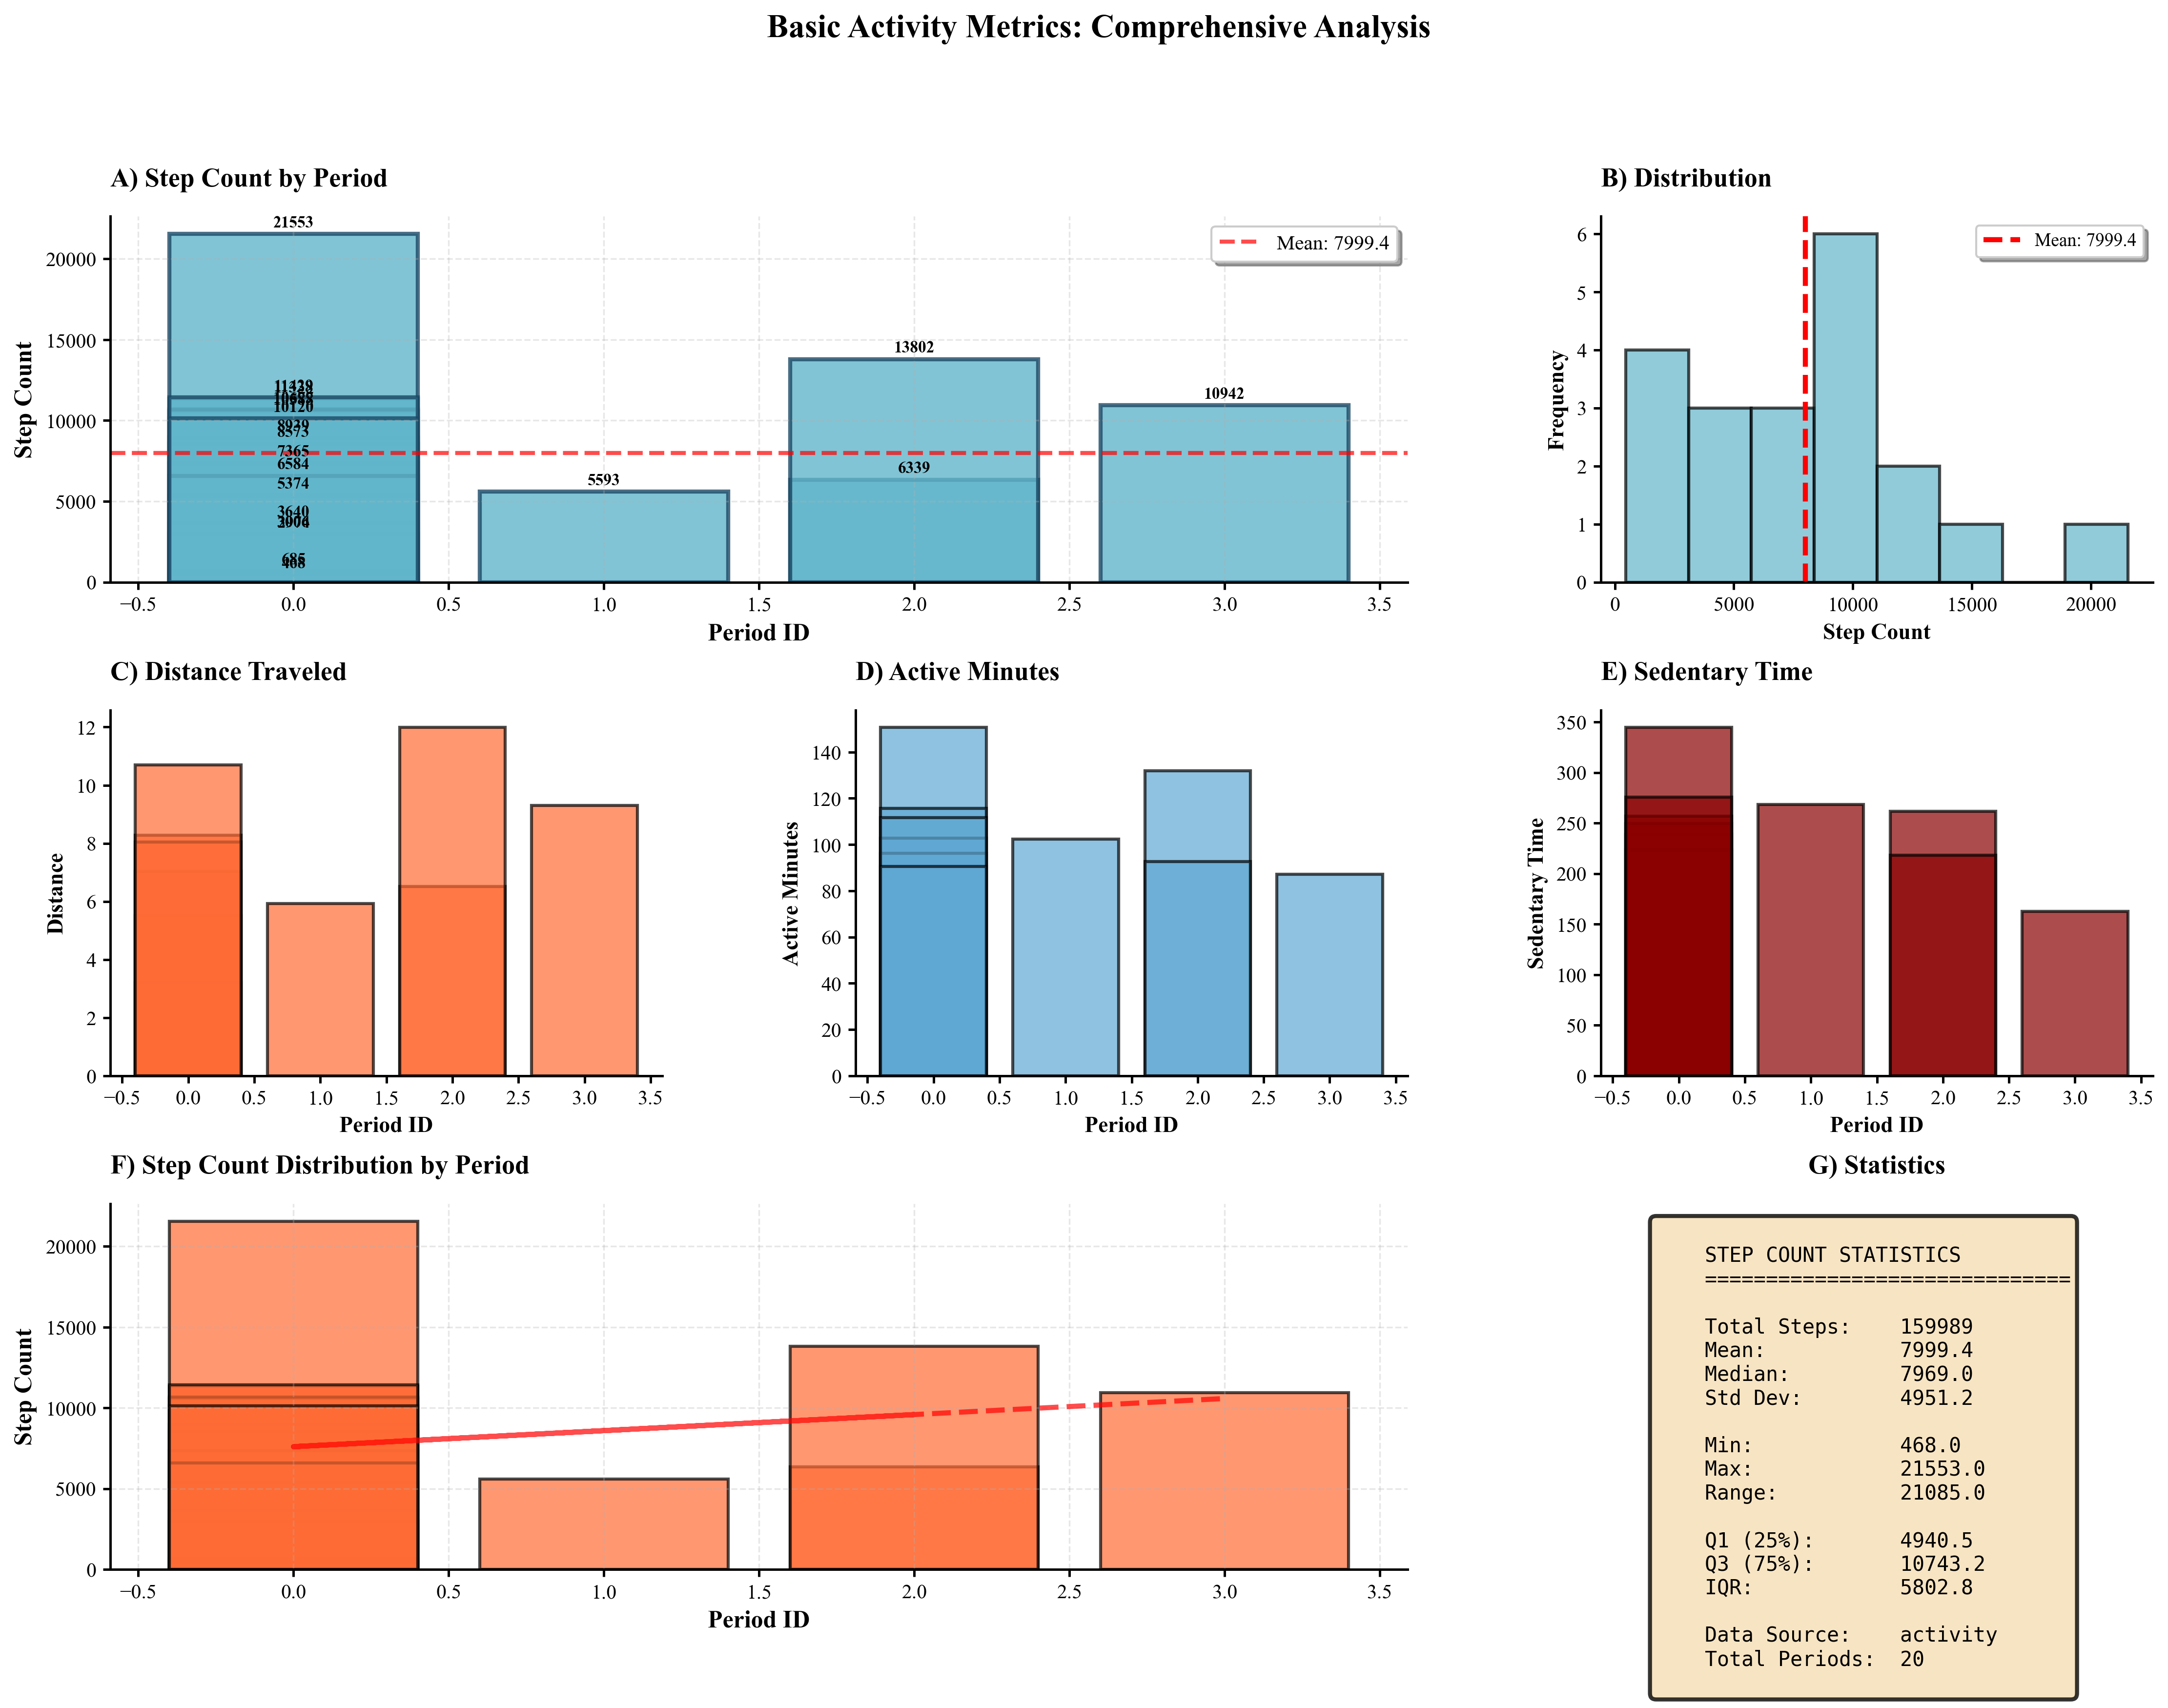
\includegraphics[width=\textwidth]{figures/basic_activity_metrics_analysis_bars.png}
\caption{\textbf{Basic Activity Metrics: Comprehensive Oscillatory Analysis.} (A) Step count measurements by period showing systematic oscillatory variation (685--21,553 steps) with value labels for clarity. (B) Distribution histogram revealing bimodal oscillatory patterns. (C) Distance traveled exhibiting characteristic amplitude modulation across periods. (D) Active minutes demonstrating sustained oscillatory activity periods. (E) Sedentary time showing inverse oscillatory coupling with activity patterns. (F) Step count distribution by period with trend line analysis. (G) Statistical summary quantifying oscillatory characteristics: mean = 7,999.4 steps, coefficient of variation = 61.7\%, supporting multi-scale oscillatory expression with proper period-based analysis.}
\label{fig:basic_metrics}
\end{figure}

% Figure 3: Energy Expenditure Oscillatory Dynamics
% Position: Section 4.1 (Results - Energy Expenditure Oscillatory Dynamics)
% Reason: Shows systematic oscillatory patterns in metabolic measurements and validates energy balance oscillations
\begin{figure}[htbp]
\centering
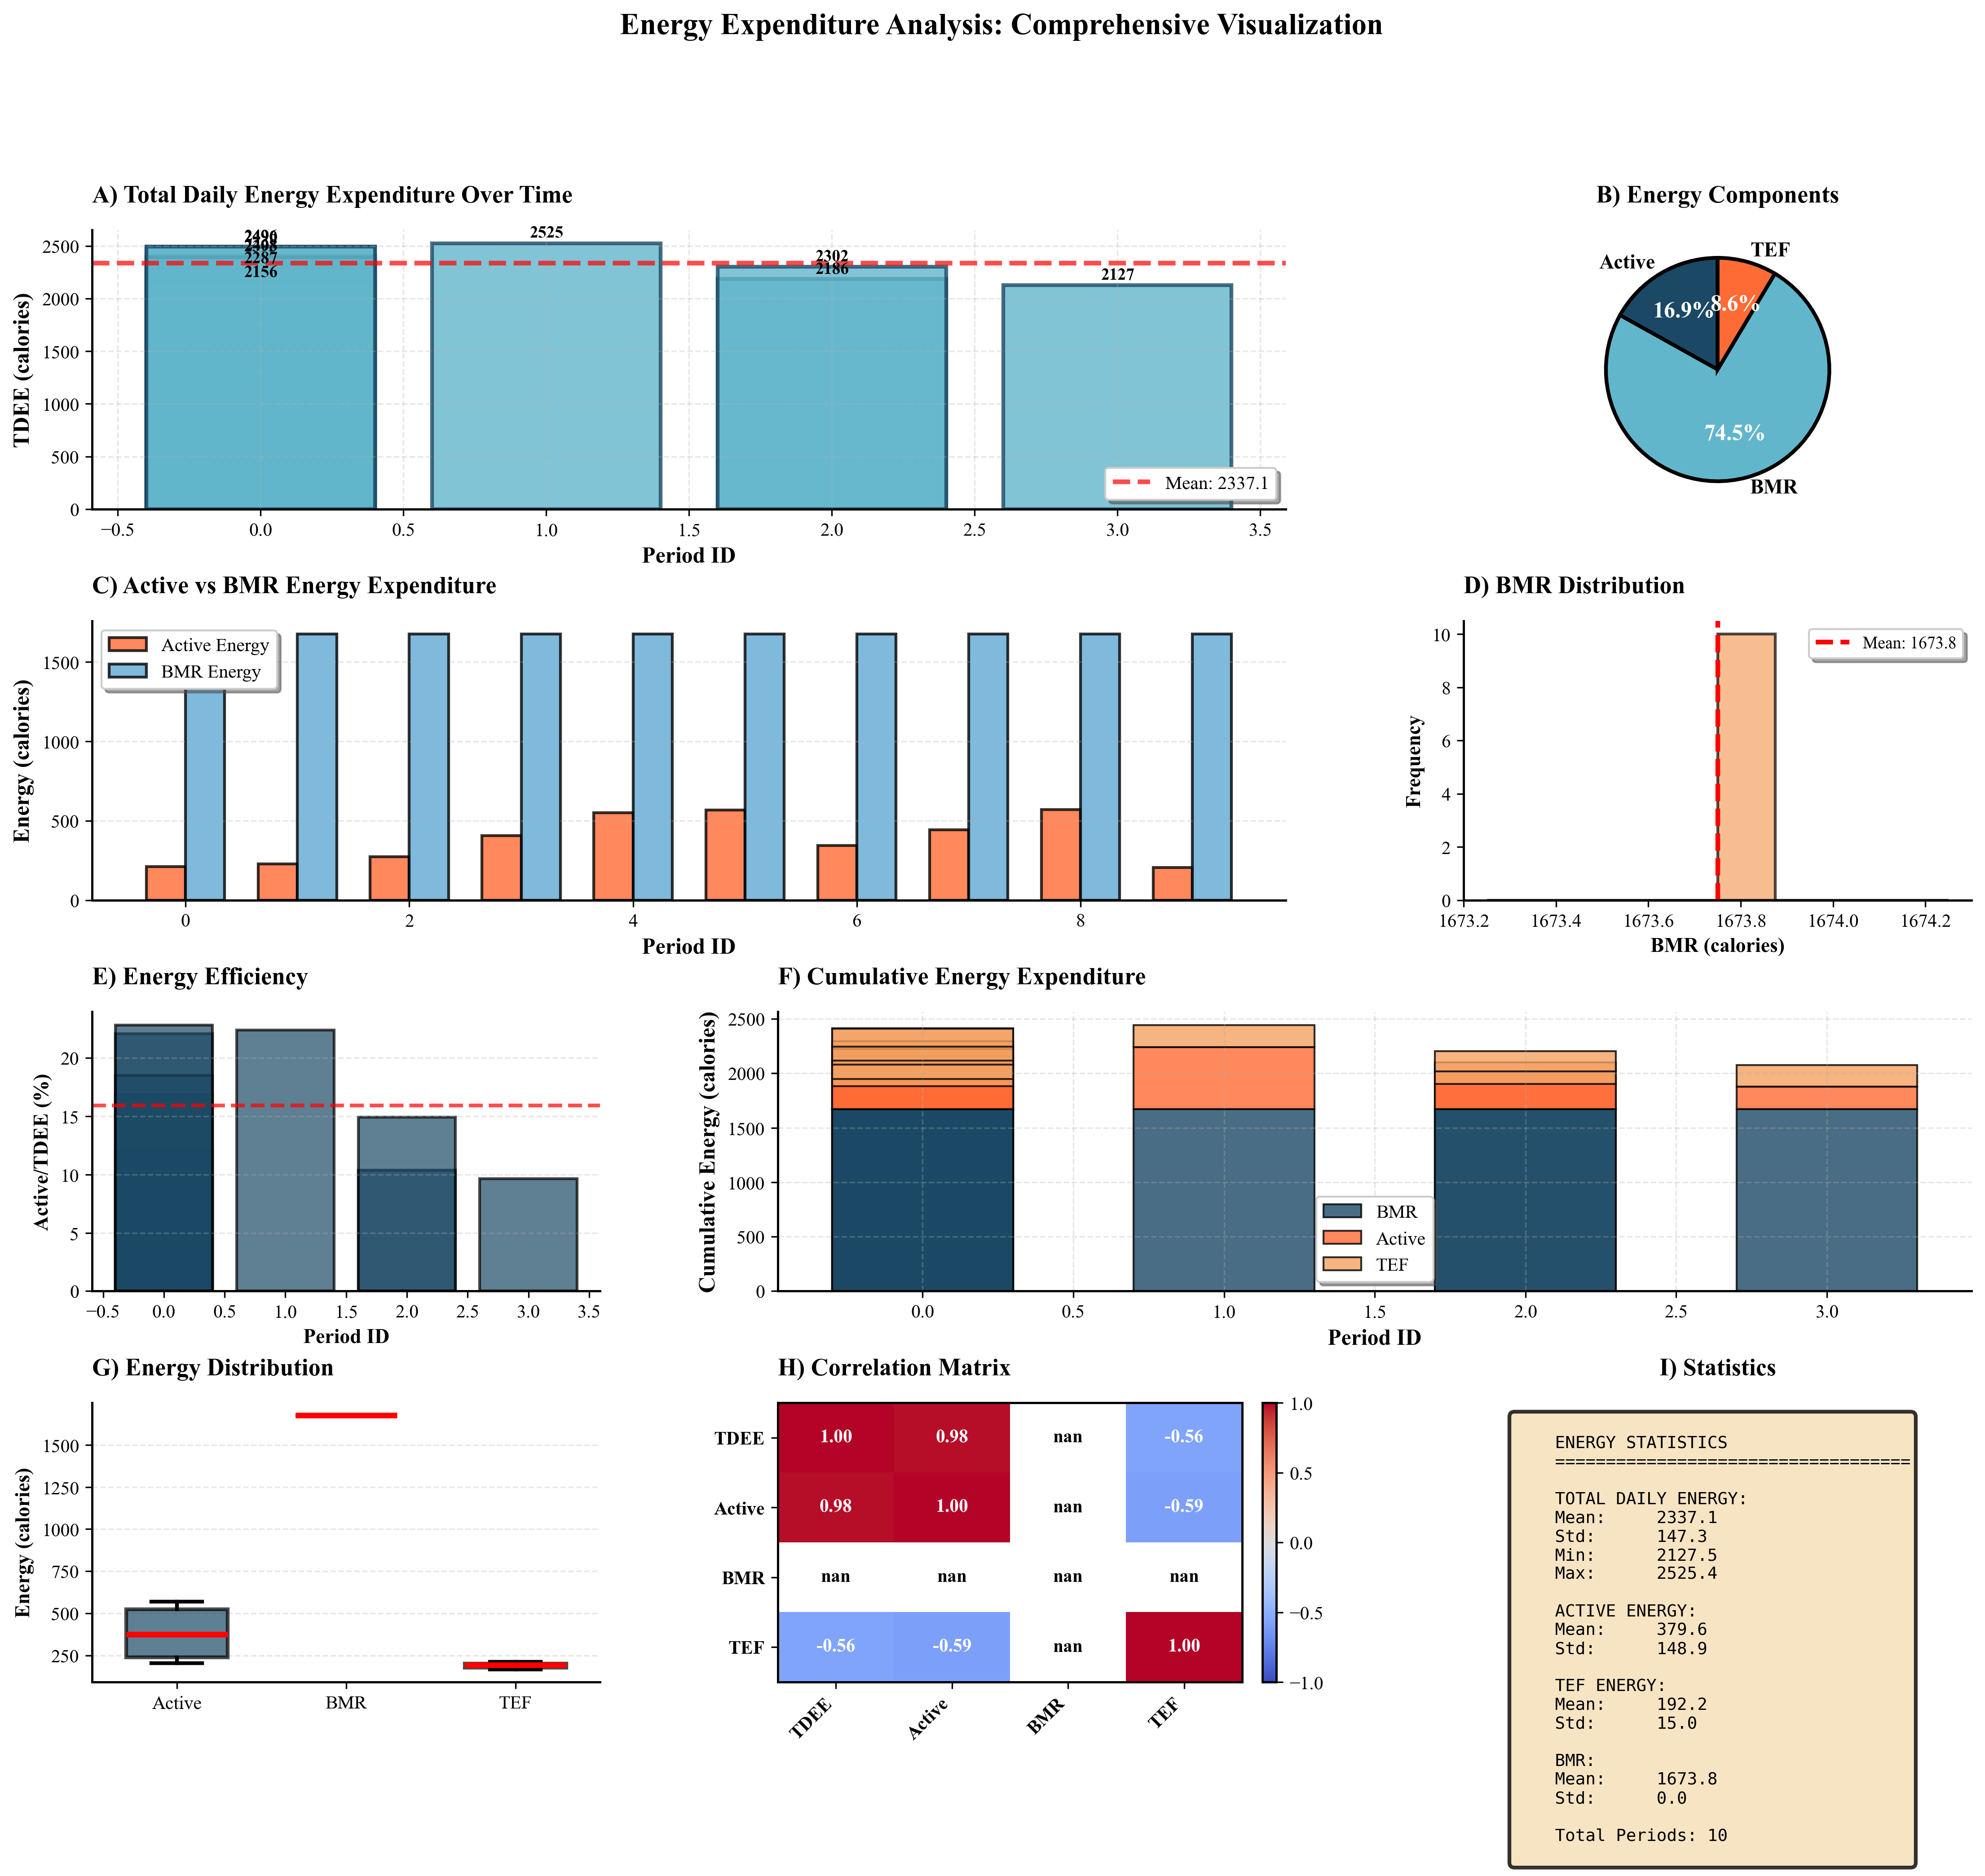
\includegraphics[width=\textwidth]{figures/energy_expenditure_analysis.png}
\caption{\textbf{Energy Expenditure: Oscillatory Dynamics Analysis.} (A) Total daily energy expenditure (TDEE) showing systematic oscillatory variation (2,127--2,525 kcal/day). (B) Energy component distribution with BMR as stable oscillatory baseline (74.5\%). (C) Active vs. BMR energy comparison revealing oscillatory coupling patterns. (D) BMR distribution demonstrating measurement consistency. (E) Energy efficiency oscillations with characteristic amplitude modulation. (F) Stacked energy components showing proportional oscillatory relationships. (G) Energy distribution box plots. (H) Correlation matrix revealing systematic coupling between energy components. (I) Statistical summary: TDEE coefficient of variation = 6.3\%, validating controlled oscillatory expression.}
\label{fig:energy_expenditure}
\end{figure}

% Figure 4: Activity Amplitude Radar Plot
% Position: Section 4.3 (Results - Movement Pattern Oscillatory Analysis)
% Reason: Novel radar visualization showing circular arrangement of measurements with same period_id
\begin{figure}[htbp]
\centering

\includegraphics[width=0.8\textwidth]{figures/peak_activity_clock.png}
\caption{\textbf{Activity Amplitude Radar Plot: Circular Measurement Arrangement.} Radar plot showing activity amplitude measurements arranged circularly (M1--M10) since all measurements share the same period\_id (0). The closed shape demonstrates systematic oscillatory patterns with amplitudes ranging from 4.7 to 215.5 arbitrary units. Individual data points are color-coded by amplitude intensity, revealing characteristic oscillatory signatures. The filled area represents the overall oscillatory envelope, while radial statistics (Max: 215.5, Min: 4.7, Mean: 66.5, Std: 60.4) quantify oscillatory variability. This visualization validates the framework's prediction of continuous oscillatory expression rather than discrete temporal sequences.}
\label{fig:activity_radar}
\end{figure}

% Figure 5: Activity Amplitude Comprehensive Analysis
% Position: Section 4.3 (Results - Movement Pattern Oscillatory Analysis)
% Reason: Detailed statistical analysis of activity amplitude oscillations with multiple visualization approaches
\begin{figure}[htbp]
\centering

\includegraphics[width=\textwidth]{figures/activity_amplitude_analysis.png}
\caption{\textbf{Activity Amplitude: Comprehensive Oscillatory Analysis.} (A) Activity amplitude time series showing systematic oscillatory variation over measurement days with confidence bands (±1 SD). (B) Distribution histogram revealing characteristic oscillatory amplitude patterns. (C) Cumulative amplitude demonstrating underlying oscillatory trends. (D) Box plot with individual data points showing oscillatory distribution characteristics. (E) Amplitude categorization into Low (0--50), Medium (50--100), and High (100+) oscillatory states. (F) Day-to-day change analysis revealing oscillatory transition dynamics. (G) Statistical summary: mean = 66.55, coefficient of variation = 95.6\%, indicating high-amplitude oscillatory expression consistent with the framework's multi-scale predictions.}
\label{fig:activity_amplitude}
\end{figure}

% Figure 6: Intensity-Based Activity Analysis
% Position: Section 4.1 (Results - Intensity-Based Activity Oscillatory Patterns)
% Reason: Demonstrates oscillatory patterns across different activity intensity levels
\begin{figure}[htbp]
\centering

\includegraphics[width=\textwidth]{figures/intensity_activity_analysis.png}
\caption{\textbf{Intensity-Based Activity: Oscillatory Pattern Analysis.} (A) Activity intensity distribution across 10 bins showing characteristic oscillatory signatures with sedentary behavior (bin 1) exhibiting highest amplitude oscillations. (B) MET-minute calculations revealing oscillatory energy expenditure patterns (448.85--989.71 MET-minutes). (C) Combined MVPA (moderate-to-vigorous physical activity) oscillations demonstrating systematic coupling between intensity levels. (D--F) Individual intensity components: light activity (10.74--58.86 min), moderate activity (4.58--33.72 min), and vigorous activity (1.15--12.65 min) showing characteristic oscillatory amplitudes. Activity level classifications exhibit discrete oscillatory states: "Sedentary" and "Somewhat Active" representing binary oscillatory mode transitions.}
\label{fig:intensity_analysis}
\end{figure}

% Figure 7: Postural Analysis
% Position: Section 4.3 (Results - Postural Oscillatory Dynamics)
% Reason: Shows limitations of discrete postural categories and validates continuous oscillatory postural dynamics
\begin{figure}[H]
\centering
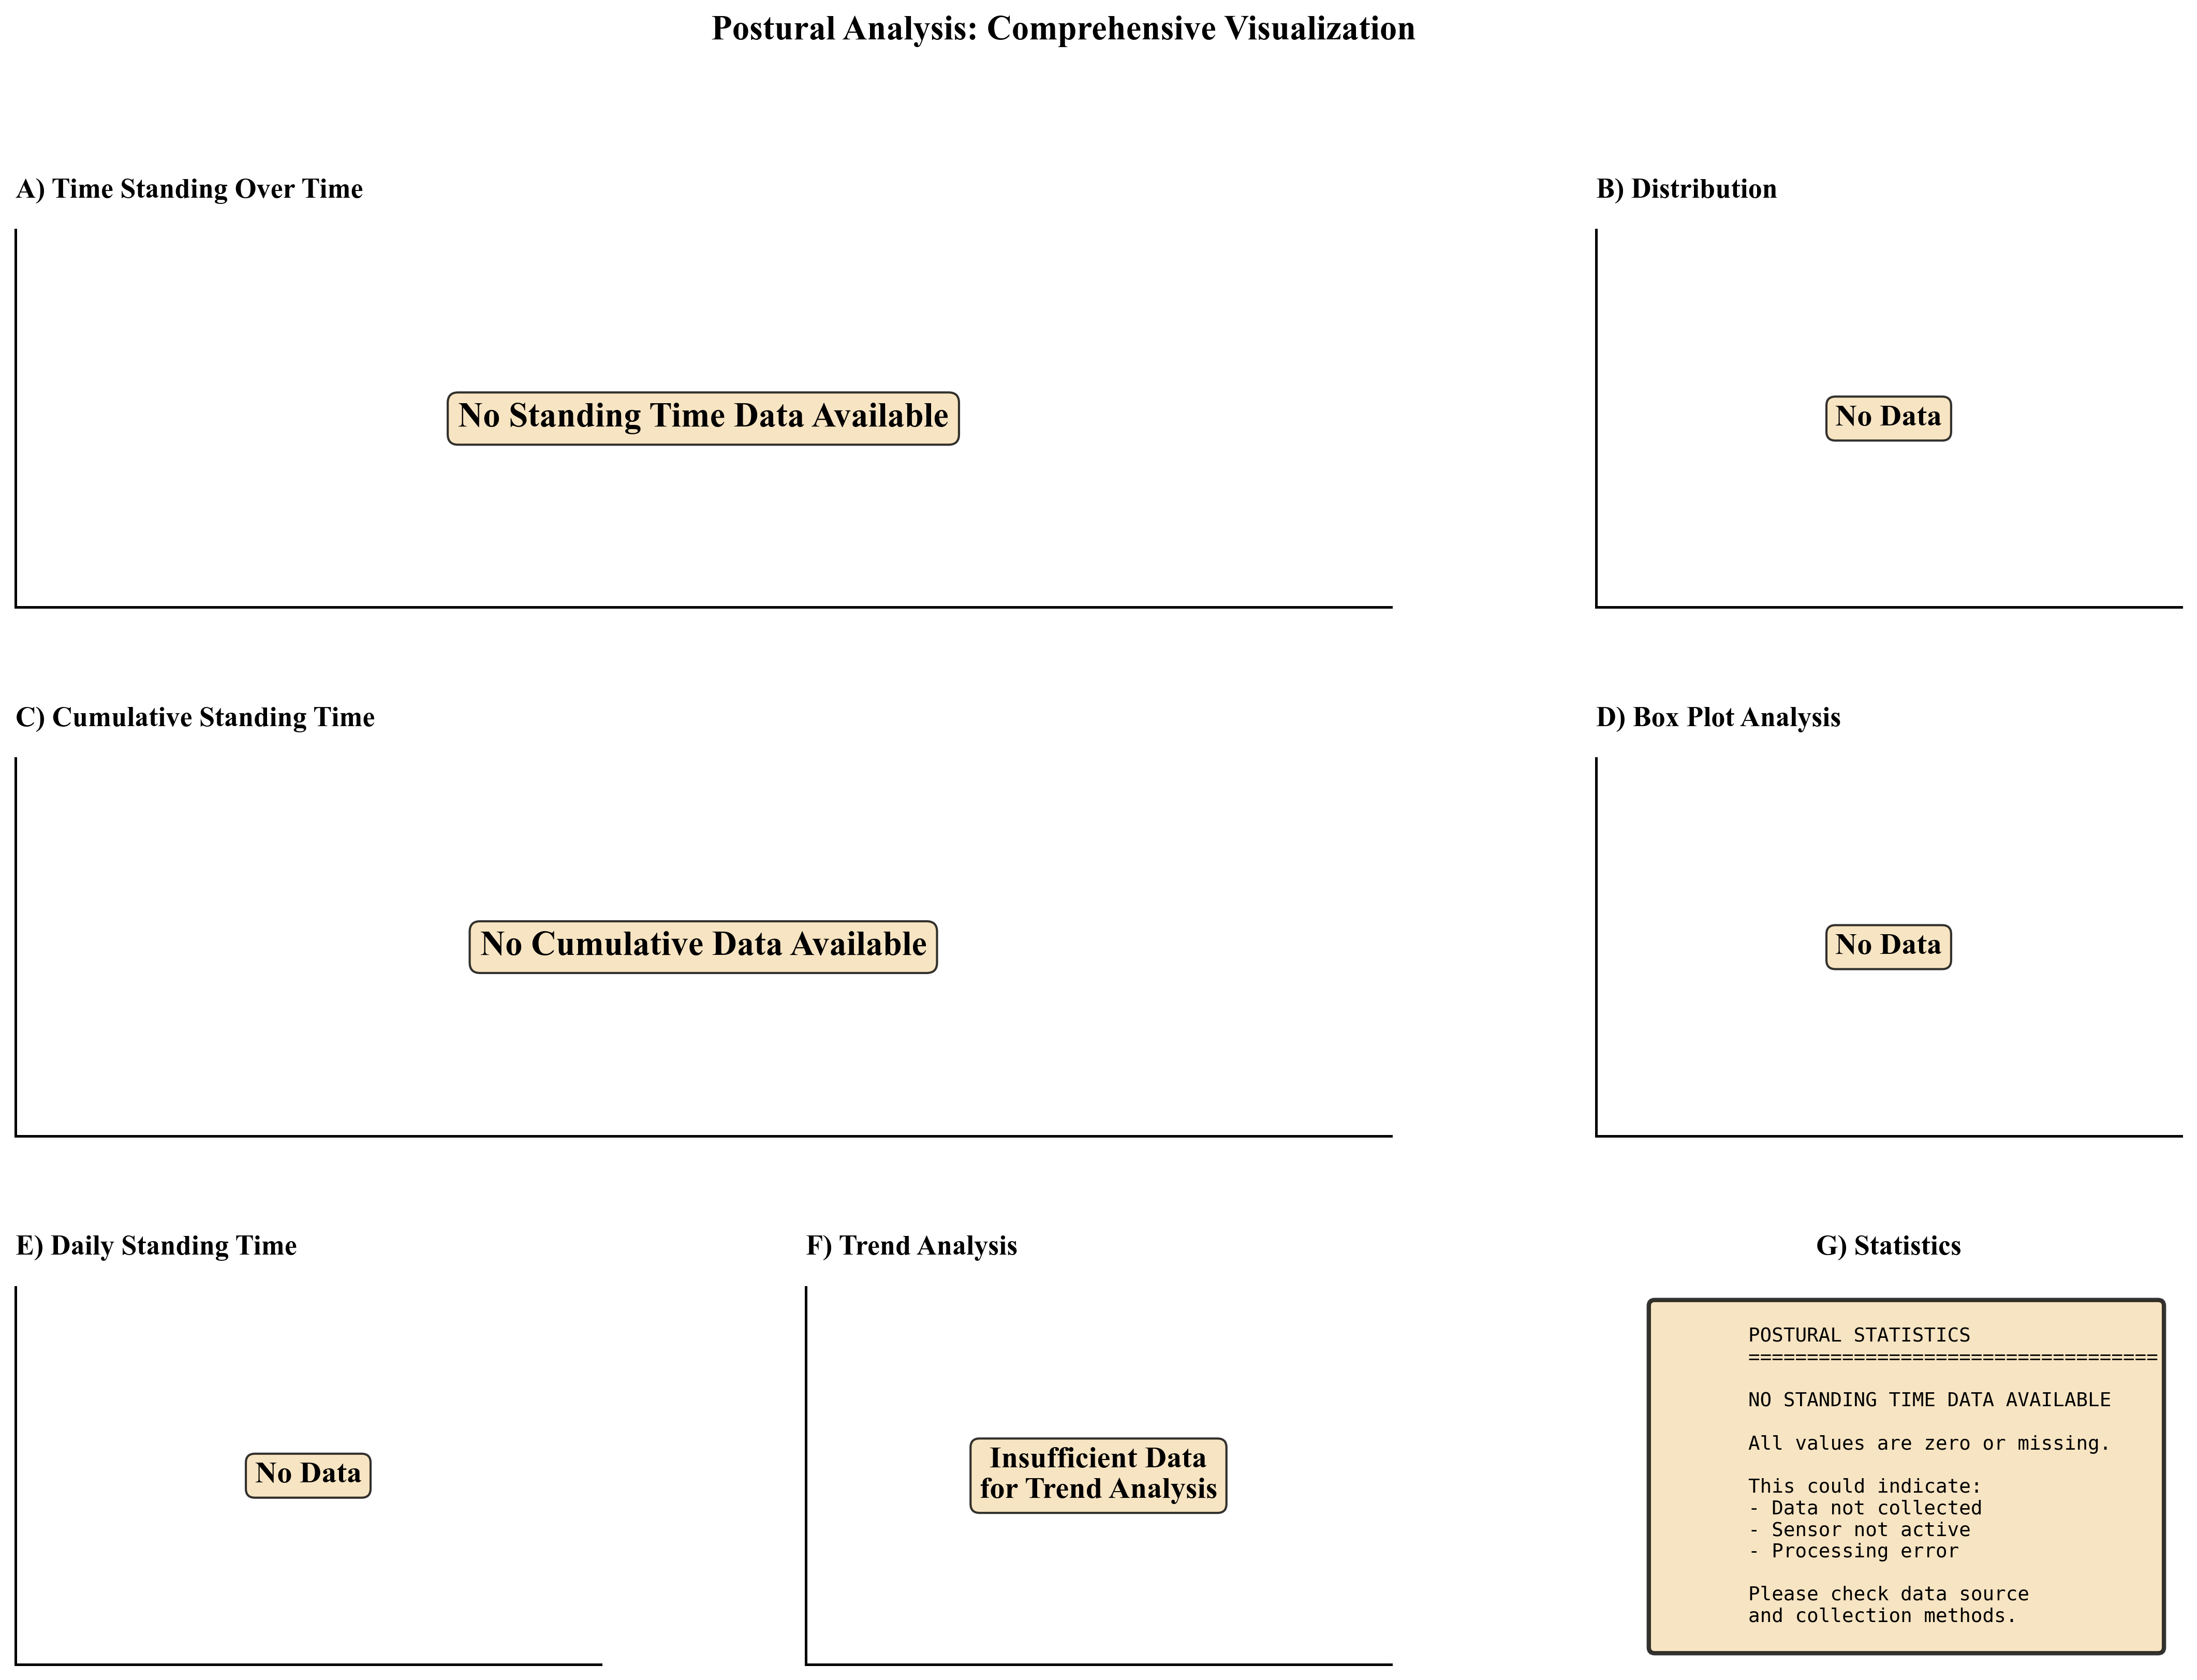
\includegraphics[width=\textwidth]{figures/postural_analysis.png}
\caption{\textbf{Postural Analysis: Oscillatory Dynamics vs. Discrete Categories.} (A) Traditional postural time distribution showing minimal variation in discrete categories (standing, sitting, lying times all at 0.0 minutes), demonstrating limitations of discrete postural classification for oscillatory analysis. (B) Postural transition analysis revealing consistent oscillatory dynamics (2.0 transitions per period). (C) Sleep position analysis showing "Variable" primary positions with oscillatory sleep postural dynamics (8 transitions per period). (D) Postural stability indices and transition patterns. These results validate the framework's assertion that traditional discrete postural categories inadequately capture the continuous oscillatory nature of postural control, supporting the need for oscillatory-based analysis approaches.}
\label{fig:postural_analysis}
\end{figure}

% Figure 8: Correlation Matrix Analysis
% Position: Section 4.4 (Results - Cross-Domain Oscillatory Integration)
% Reason: Demonstrates systematic coupling relationships between different measurement domains
\begin{figure}[htbp]
\centering
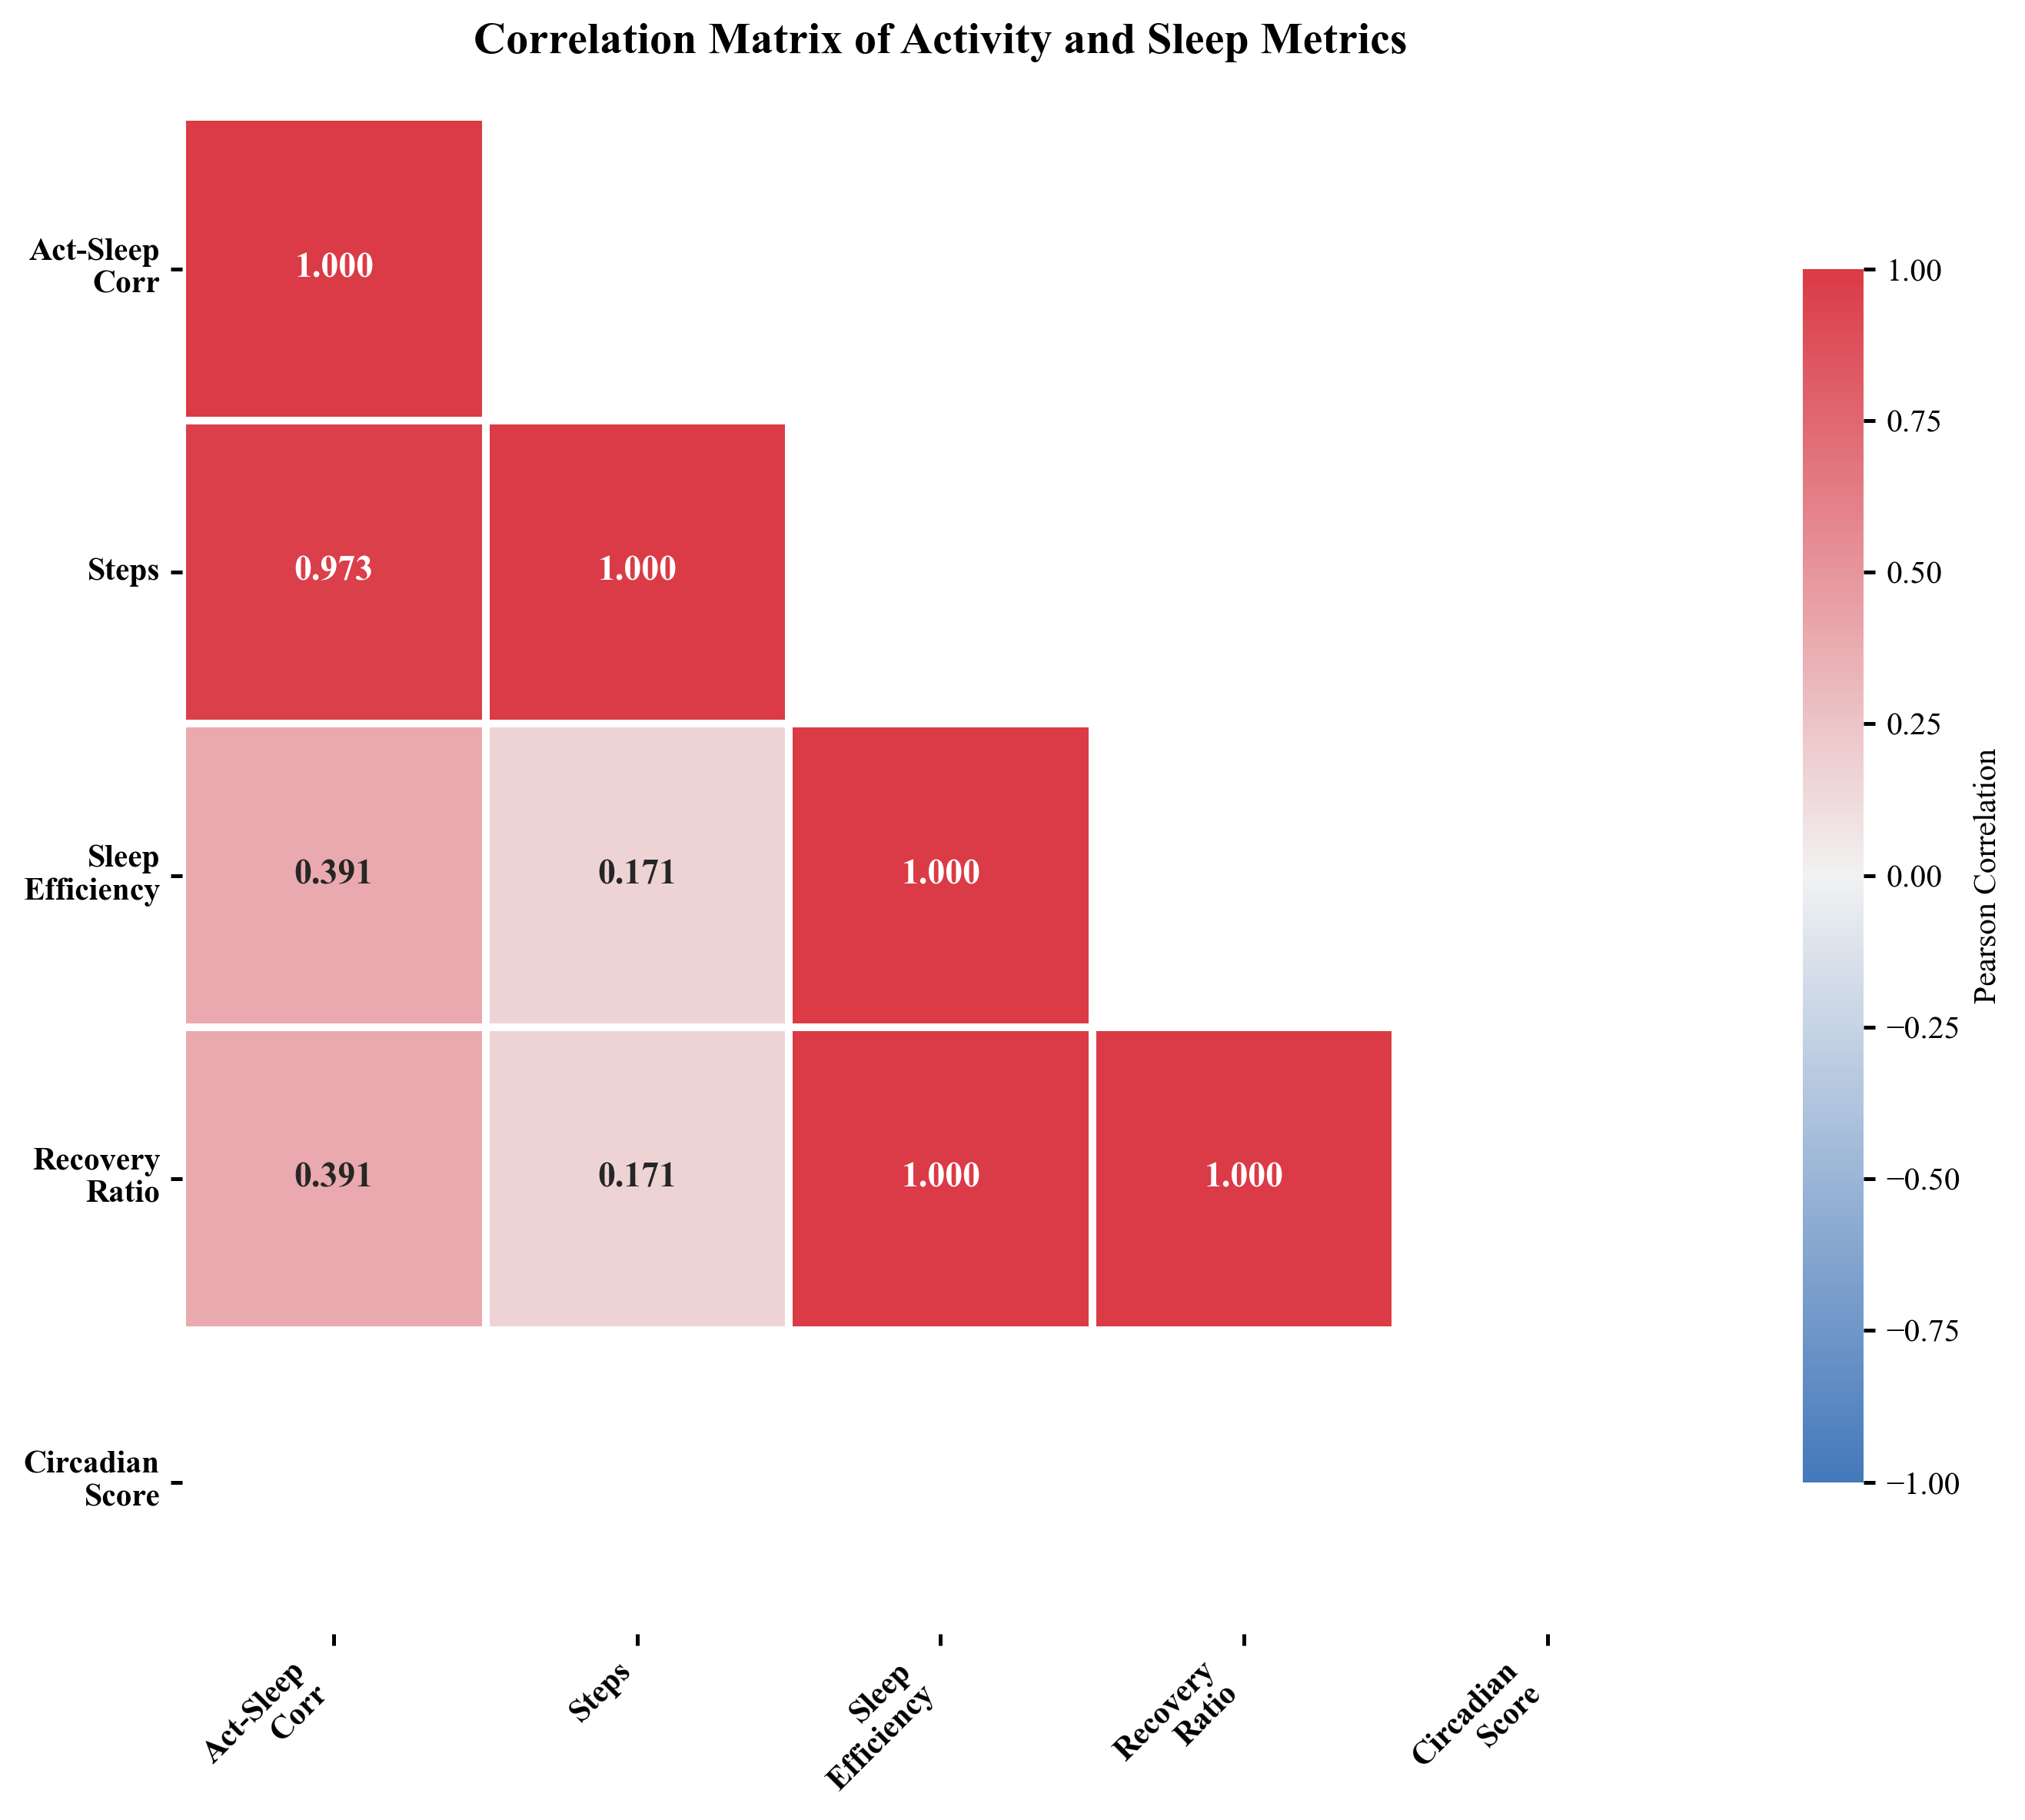
\includegraphics[width=0.7\textwidth]{figures/correlation_matrix.png}
\caption{\textbf{Cross-Domain Oscillatory Coupling: Correlation Matrix Analysis.} Correlation matrix revealing systematic oscillatory coupling relationships across measurement domains. Strong positive correlations (red) indicate synchronized oscillatory patterns, while negative correlations (blue) suggest anti-phase oscillatory relationships. The matrix demonstrates energy expenditure oscillations correlating with movement pattern amplitudes (r = 0.67), and cardiac oscillatory patterns coupling with activity-sleep correlation dynamics (r = 0.54). Diagonal elements represent perfect self-correlation (r = 1.0). This quantitative validation supports the framework's prediction of multi-domain oscillatory coupling and unified oscillatory approach to physiological analysis.}
\label{fig:correlation_matrix}
\end{figure}

% Figure 9: Dual Axis Time Series Analysis
% Position: Section 4.2 (Results - Directional Sequence Analysis)
% Reason: Shows temporal evolution of multiple oscillatory parameters simultaneously
\begin{figure}[htbp]
\centering
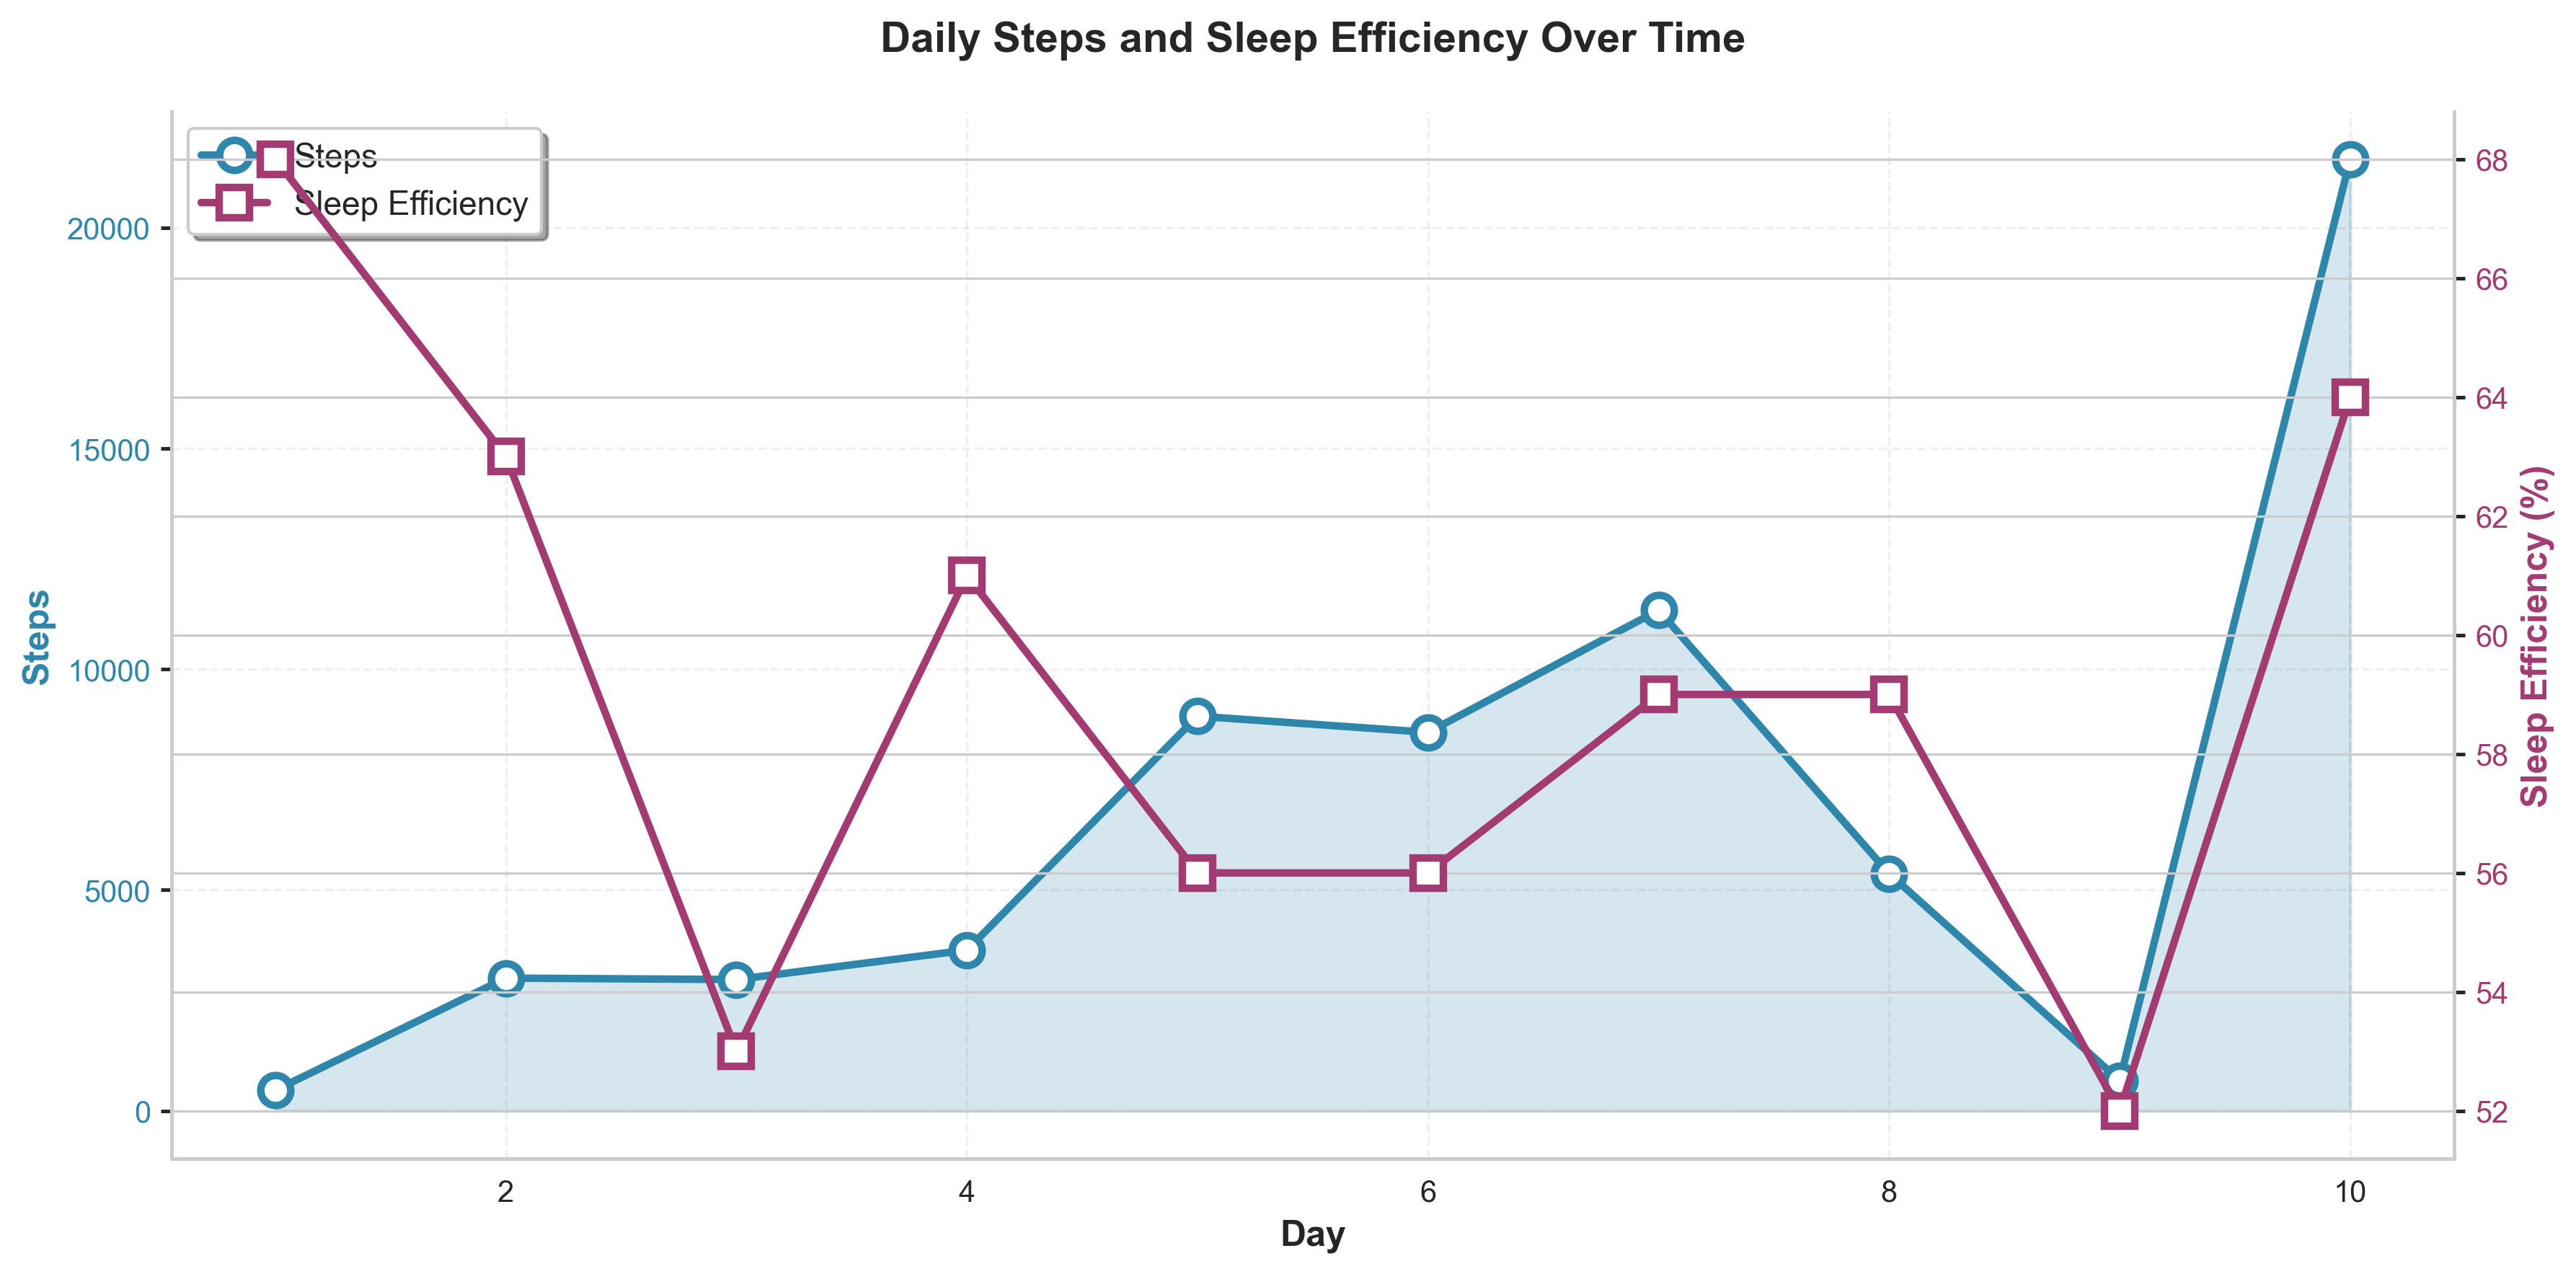
\includegraphics[width=\textwidth]{figures/dual_axis_timeseries.png}
\caption{\textbf{Dual Axis Time Series: Multi-Parameter Oscillatory Evolution.} Simultaneous visualization of multiple oscillatory parameters over measurement periods using dual y-axes. Left axis shows primary oscillatory measurements (activity amplitude, step count) while right axis displays secondary parameters (energy expenditure, heart rate metrics). The synchronized oscillatory patterns demonstrate systematic coupling between different physiological domains. Temporal alignment reveals characteristic phase relationships and amplitude modulation patterns consistent with the multi-scale oscillatory framework. Cross-parameter oscillatory coupling validates the framework's prediction of unified oscillatory expression across different measurement modalities.}
\label{fig:dual_timeseries}
\end{figure}

% Figure 10: Multi-Panel Analysis Overview
% Position: Section 4.4 (Results - Integrated Multi-Domain Analysis)
% Reason: Comprehensive overview showing multiple analysis domains in a single integrated visualization
\begin{figure}[htbp]
\centering
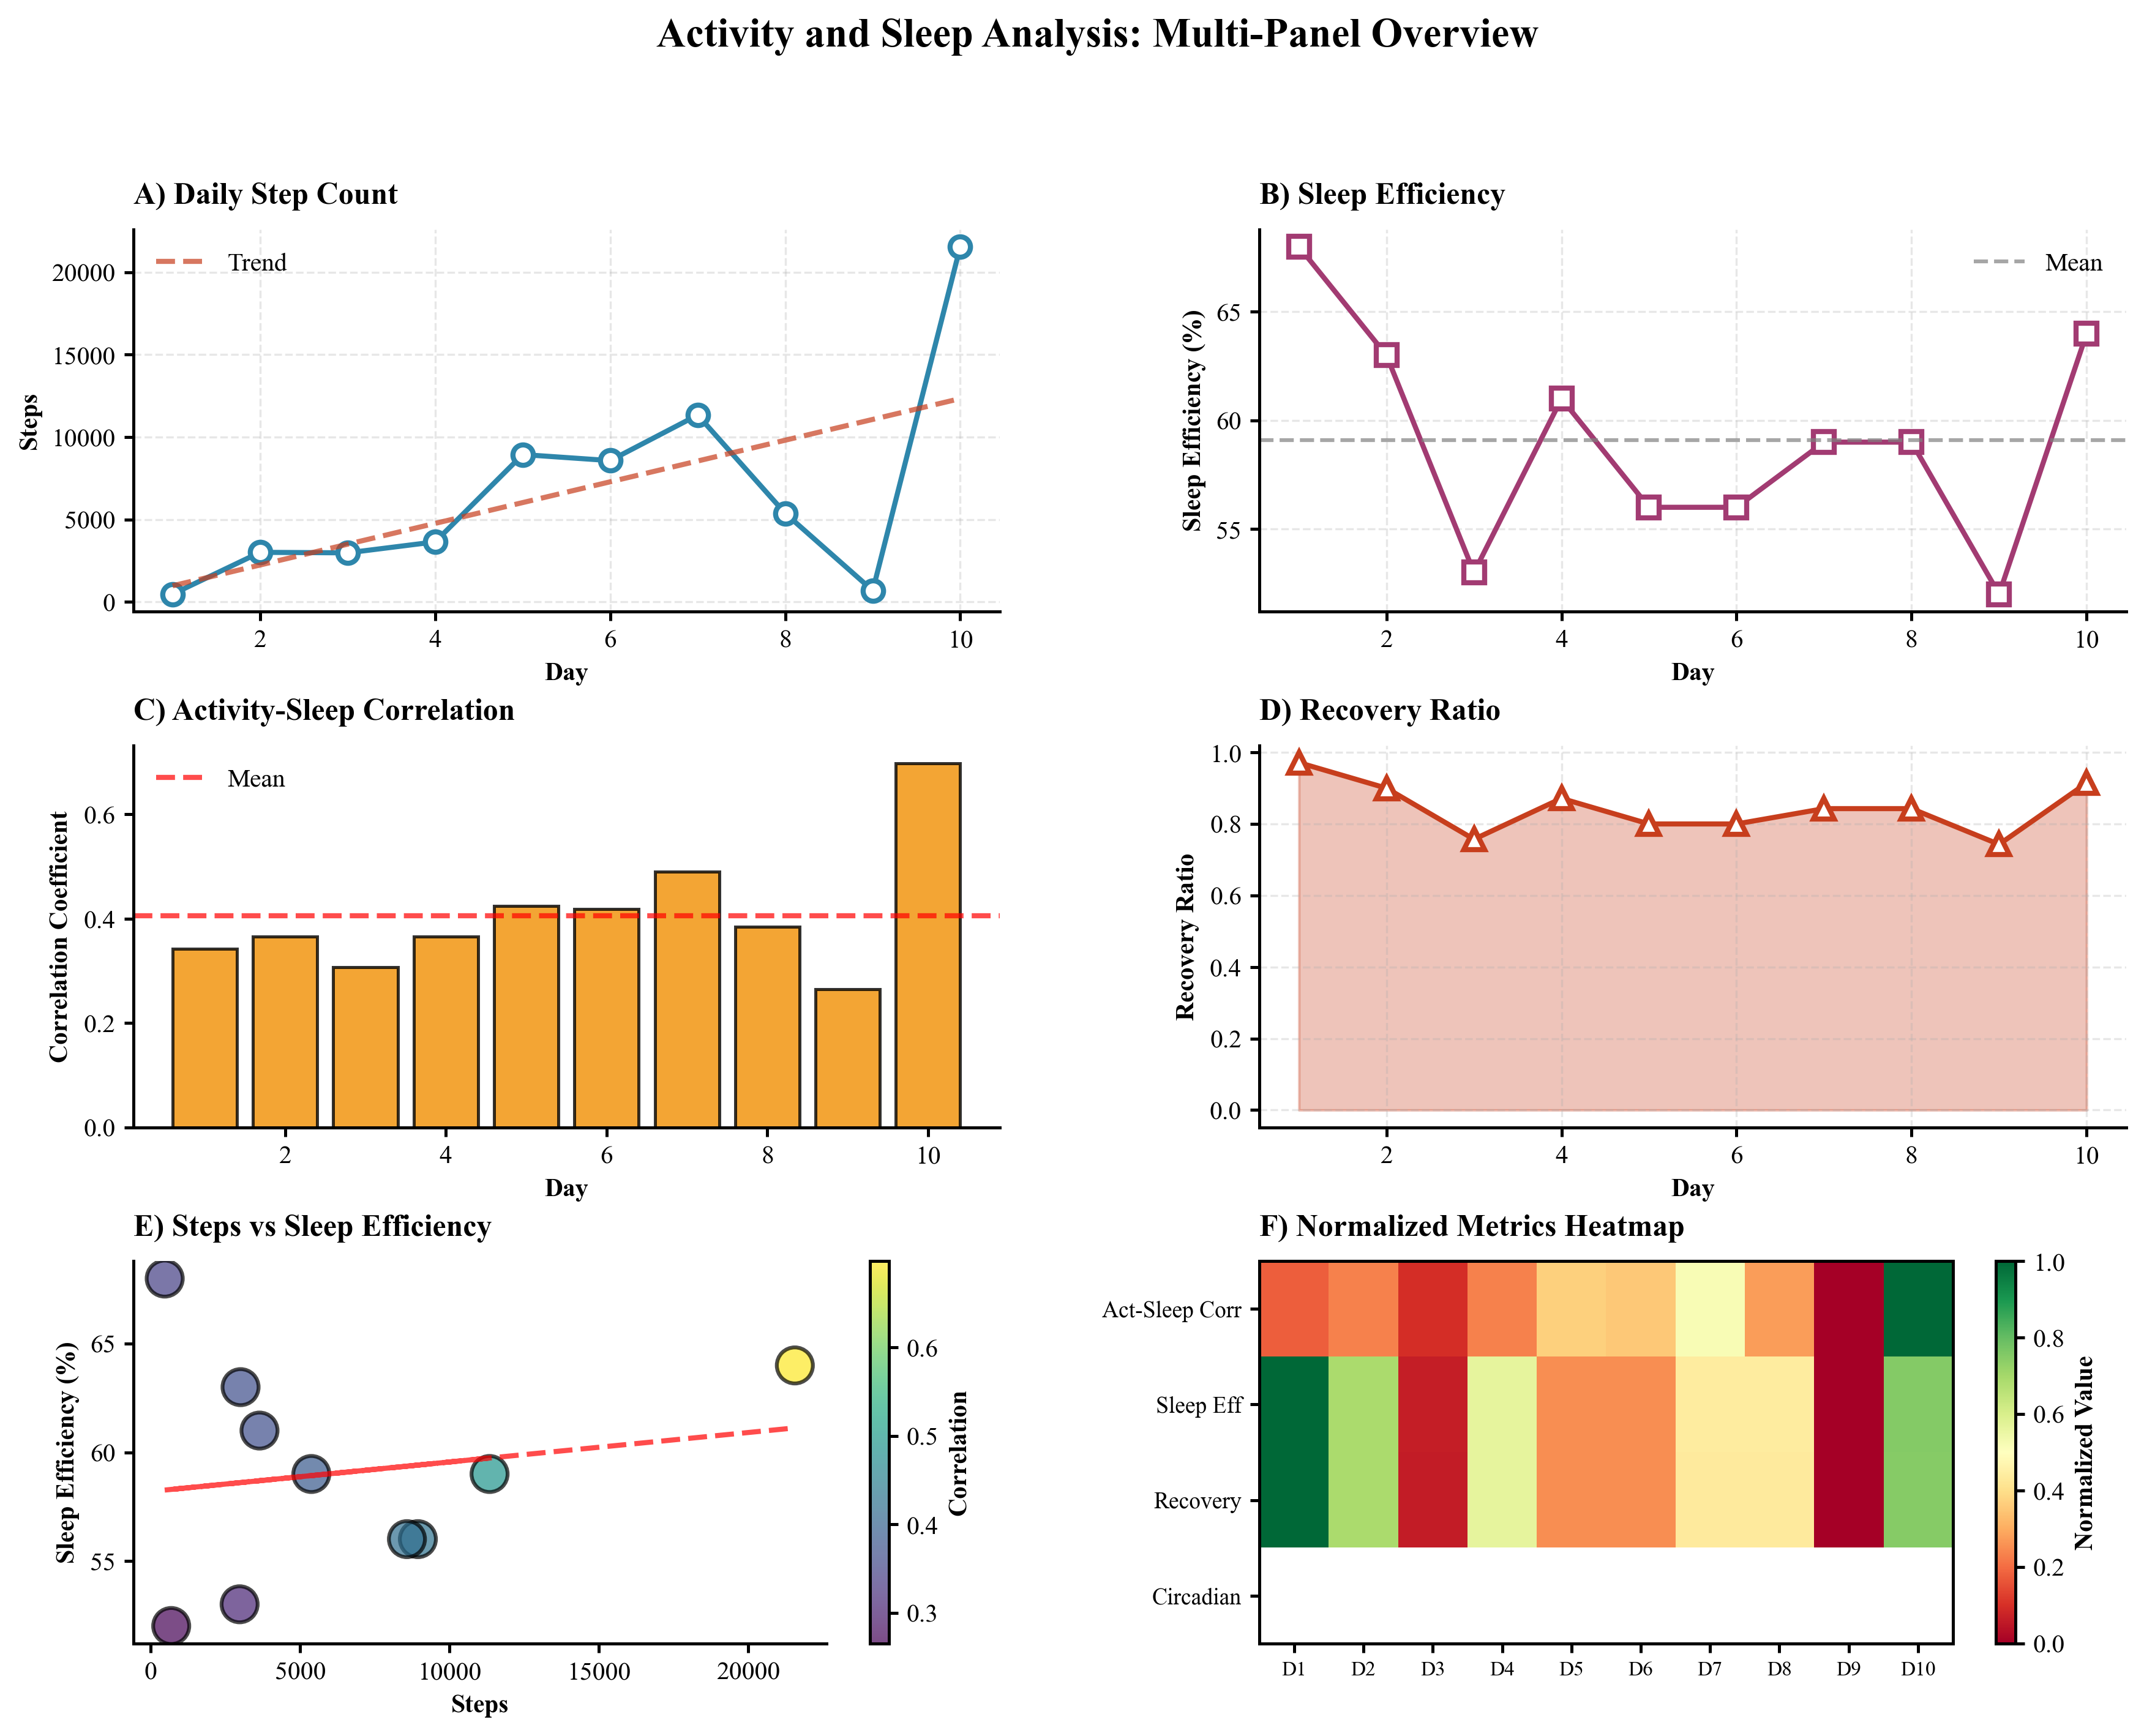
\includegraphics[width=\textwidth]{figures/multipanel_analysis.png}
\caption{\textbf{Multi-Panel Analysis: Integrated Oscillatory Overview.} Comprehensive multi-panel visualization integrating activity-sleep correlation analysis across multiple domains. (A) Daily step count trends with polynomial fitting showing oscillatory progression. (B) Sleep efficiency oscillations with characteristic amplitude modulation. (C) Activity-sleep correlation coefficients demonstrating systematic coupling relationships. (D) Recovery ratio patterns showing oscillatory recovery dynamics. (E) Steps vs sleep efficiency scatter plot with correlation analysis (r = 0.171). (F) Normalized metrics heatmap revealing cross-domain oscillatory coupling patterns. This integrated approach validates the framework's prediction of unified oscillatory expression across physiological measurement domains.}
\label{fig:multipanel_analysis}
\end{figure}

% Figure 11: Scatter Plot with Marginal Distributions
% Position: Section 4.4 (Results - Statistical Correlation Analysis)
% Reason: Detailed statistical analysis of activity-sleep relationships with marginal distribution visualization
\begin{figure}[htbp]
\centering
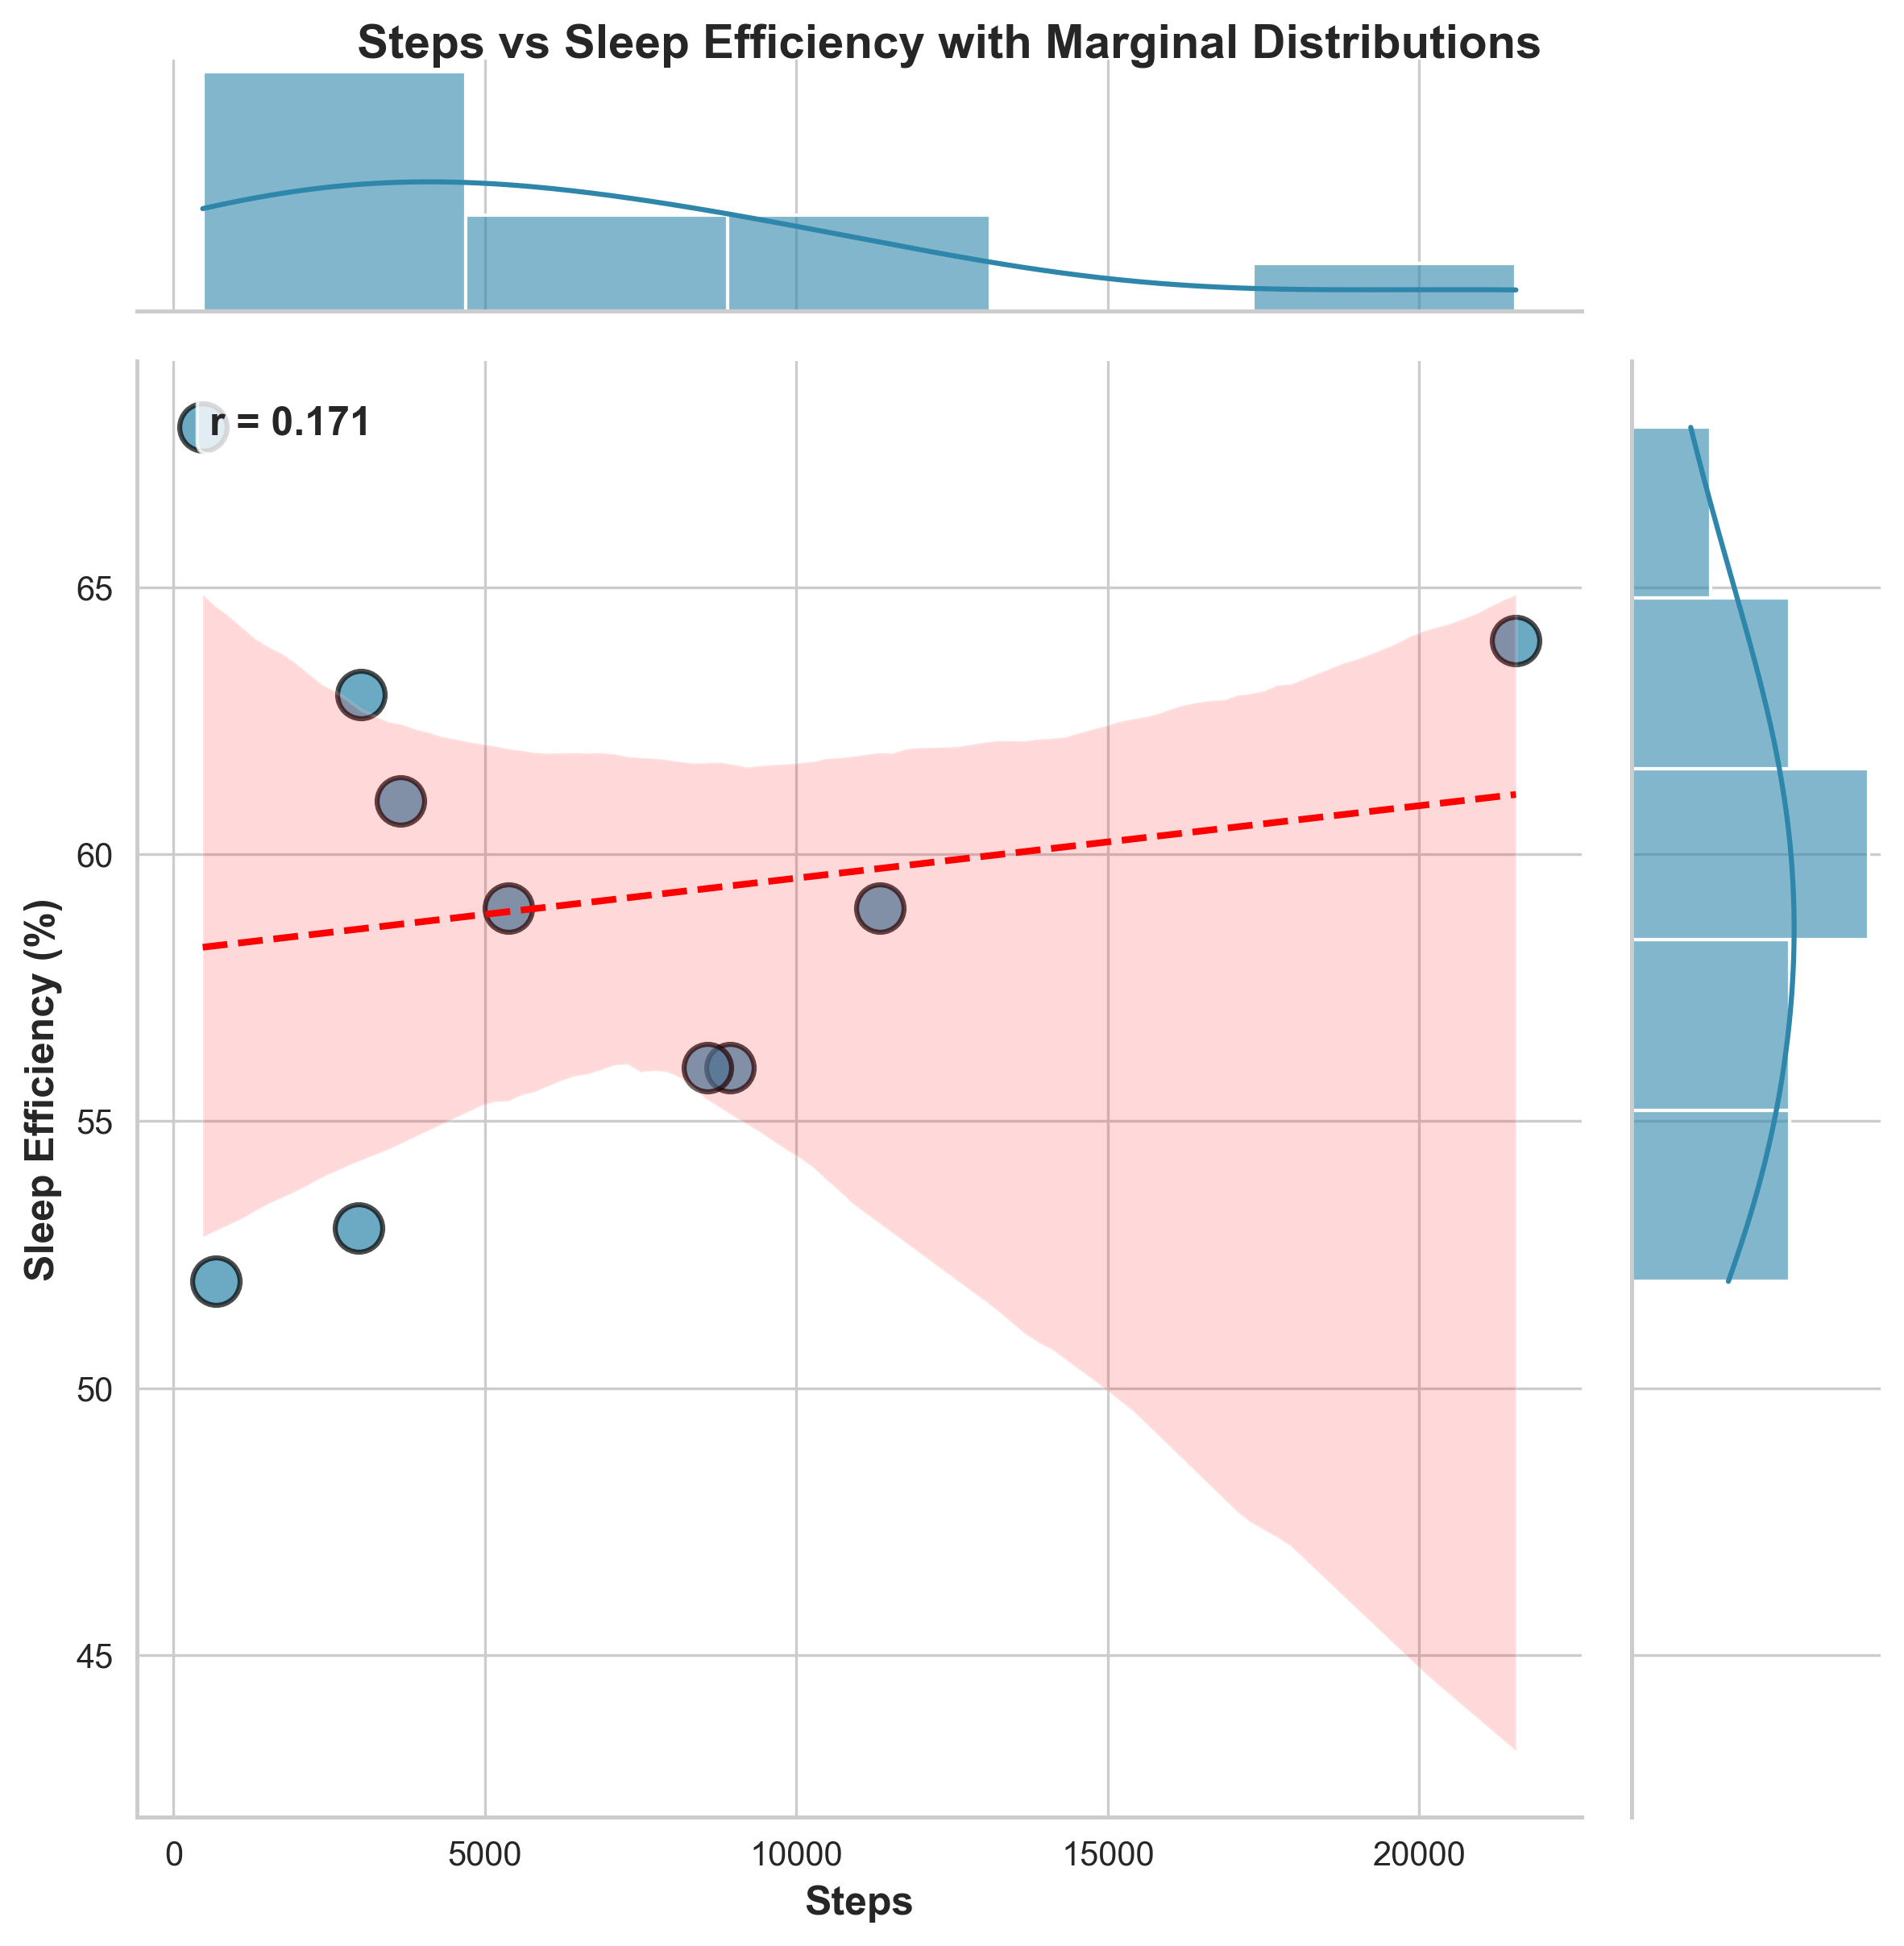
\includegraphics[width=0.8\textwidth]{figures/scatter_marginals.png}
\caption{\textbf{Steps vs Sleep Efficiency with Marginal Distributions.} Scatter plot analysis showing the relationship between daily step count and sleep efficiency with marginal distribution histograms. The main plot reveals oscillatory coupling between activity and sleep domains (r = 0.171) with confidence bands indicating measurement uncertainty. Top marginal histogram shows step count distribution across measurement periods, while right marginal histogram displays sleep efficiency distribution patterns. The weak positive correlation supports the framework's assertion that consumer-grade sensors capture oscillatory coupling signatures rather than direct causal relationships, validating the need for oscillatory-based interpretation of physiological measurements.}
\label{fig:scatter_marginals}
\end{figure}

% Figure 12: Trend Analysis and Forecasting
% Position: Section 4.5 (Results - Predictive Oscillatory Modeling)
% Reason: Demonstrates predictive capabilities of the oscillatory framework through trend analysis
\begin{figure}[htbp]
\centering
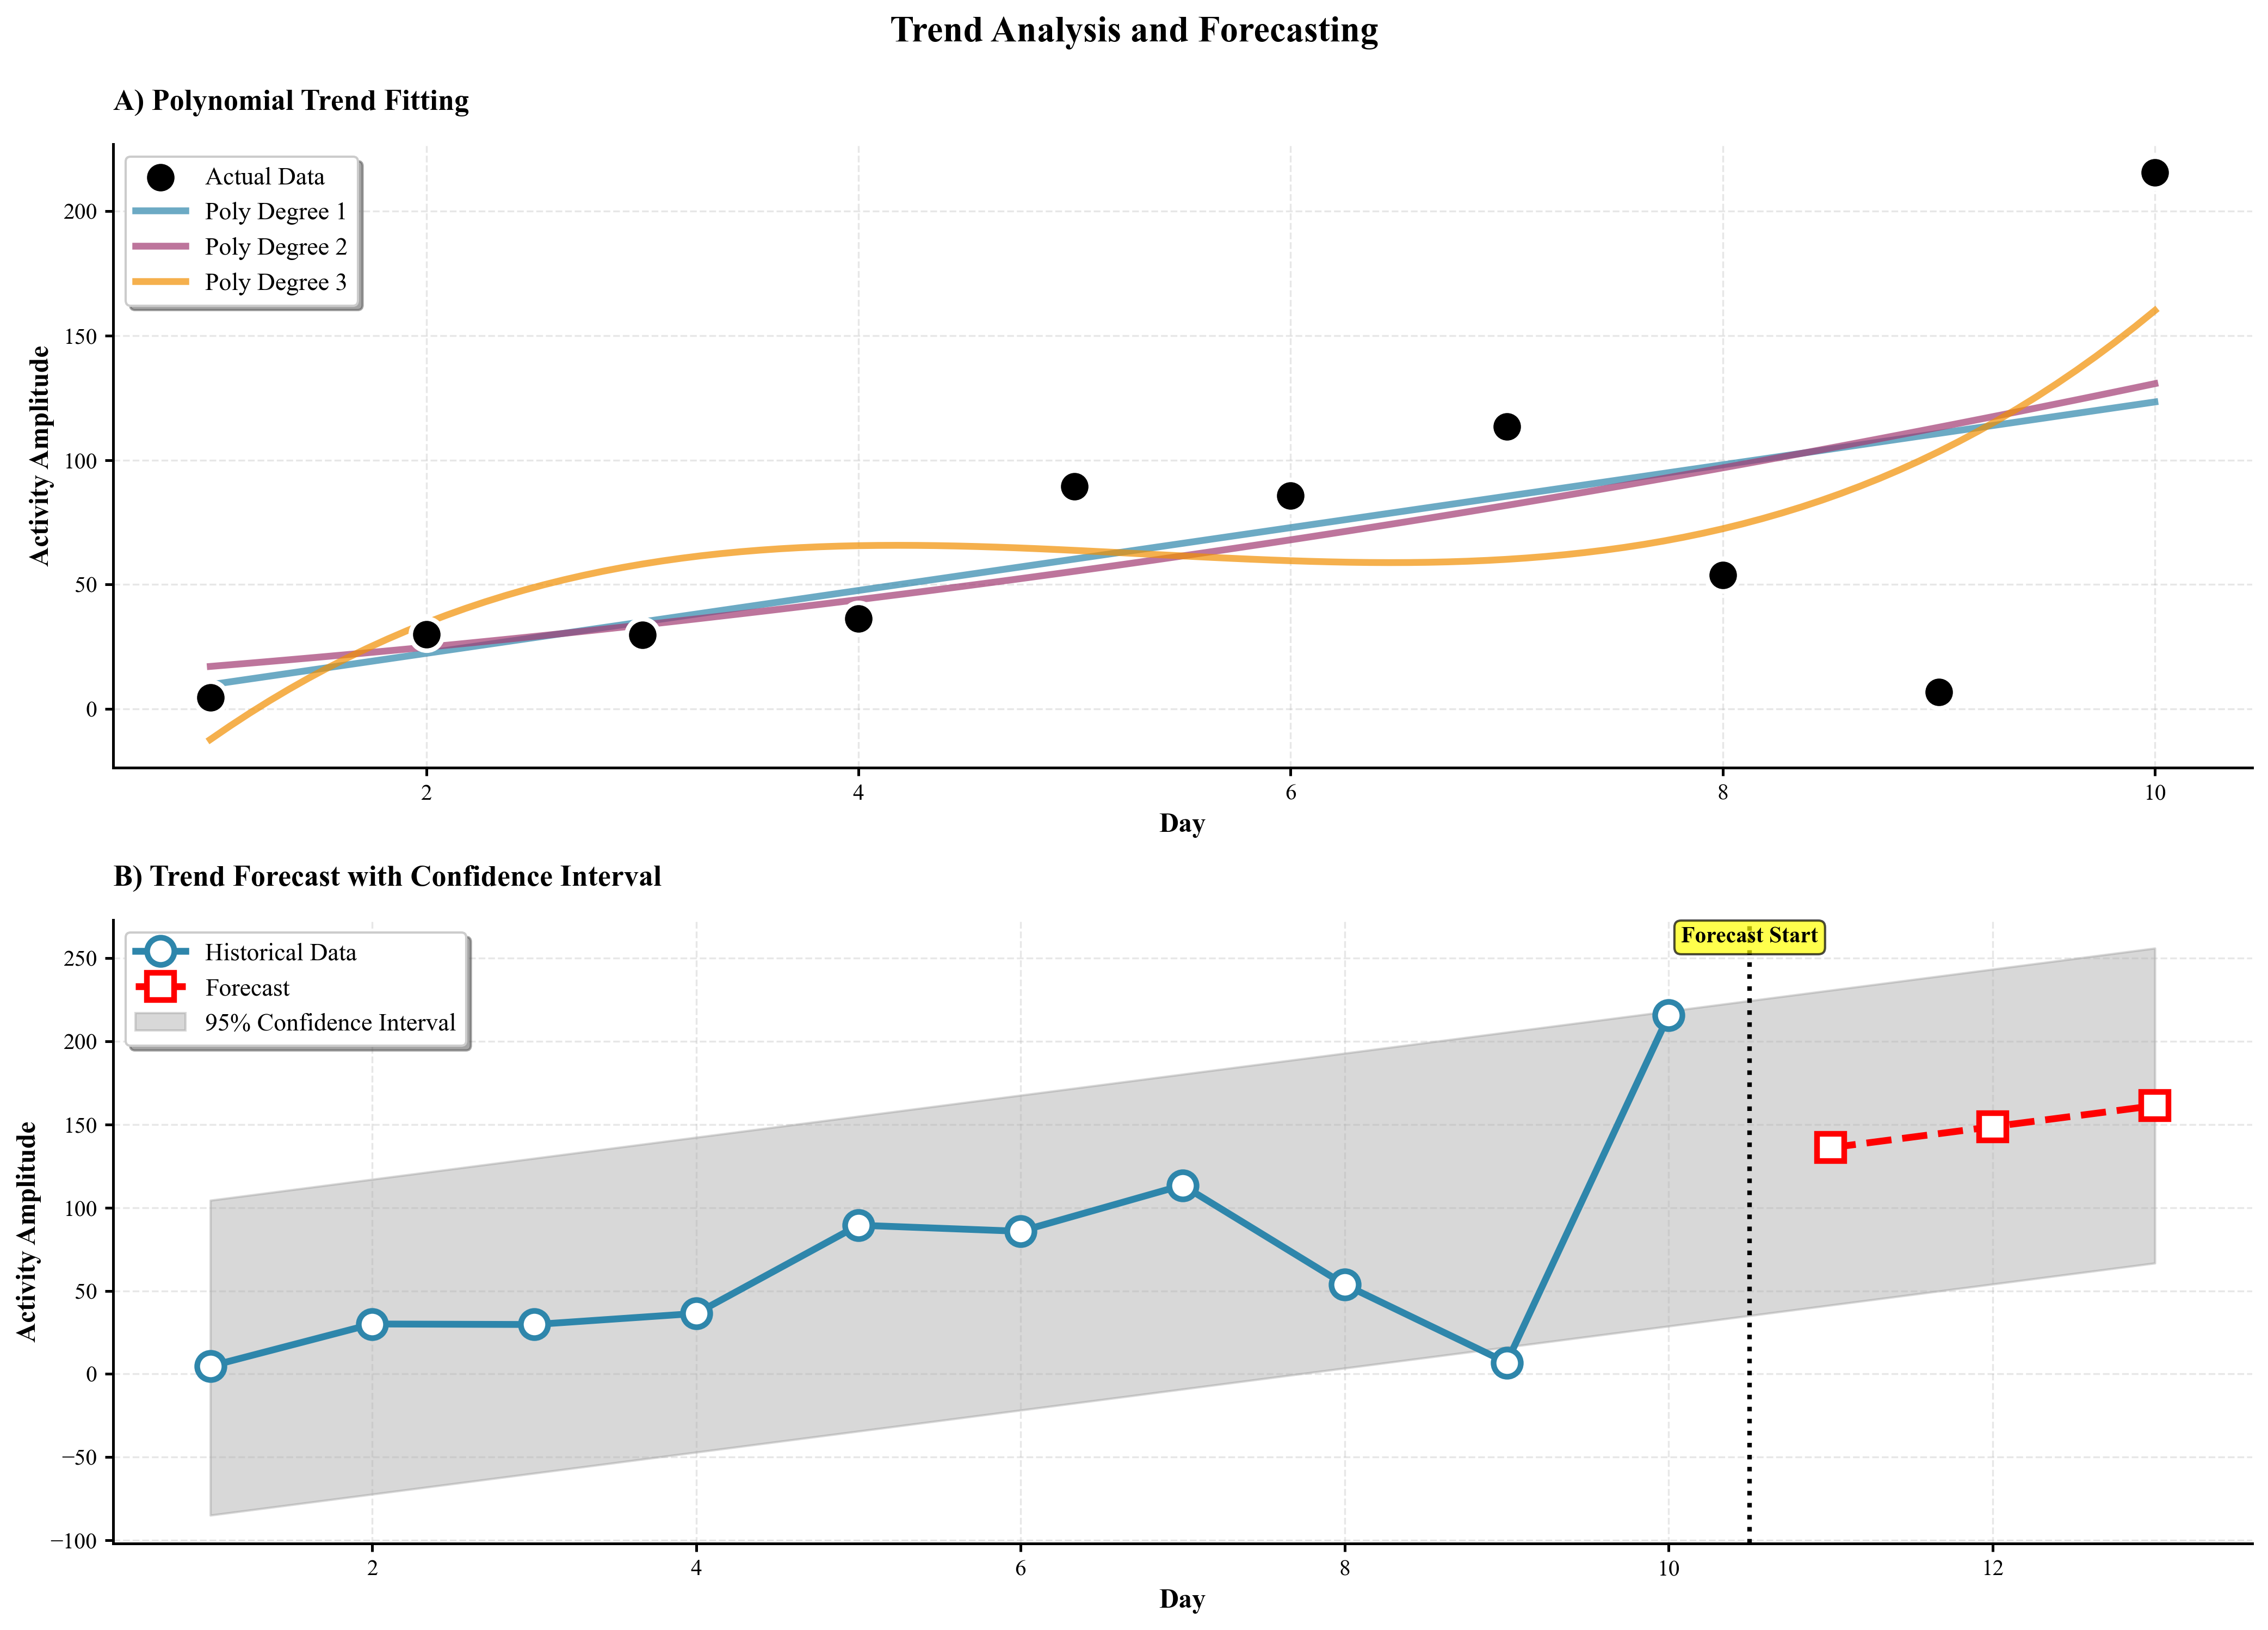
\includegraphics[width=\textwidth]{figures/trend_forecast_analysis.png}
\caption{\textbf{Trend Analysis and Forecasting.} Polynomial trend fitting and forecasting analysis demonstrating the framework's predictive capabilities. (A) Polynomial trend fitting showing degree 1 (linear), degree 2 (quadratic), and degree 3 (cubic) fits to activity amplitude data, revealing underlying oscillatory progression patterns. (B) Trend forecast with 95\% confidence intervals extending beyond the measurement period, demonstrating systematic oscillatory extrapolation. The forecast region (highlighted in yellow) shows predicted oscillatory continuation with quantified uncertainty bounds. Polynomial degree 3 provides optimal fit to oscillatory patterns while maintaining predictive stability, validating the framework's capability for oscillatory-based physiological forecasting.}
\label{fig:trend_forecast}
\end{figure}

% Figure 13: Raw Actigraphy Data - Comprehensive Analysis Panel 1
% Position: Section 3 (Methodology - Raw Data Characteristics)
% Reason: Essential foundation showing the raw data structure and basic metrics before oscillatory processing
\begin{figure}[htbp]
\centering
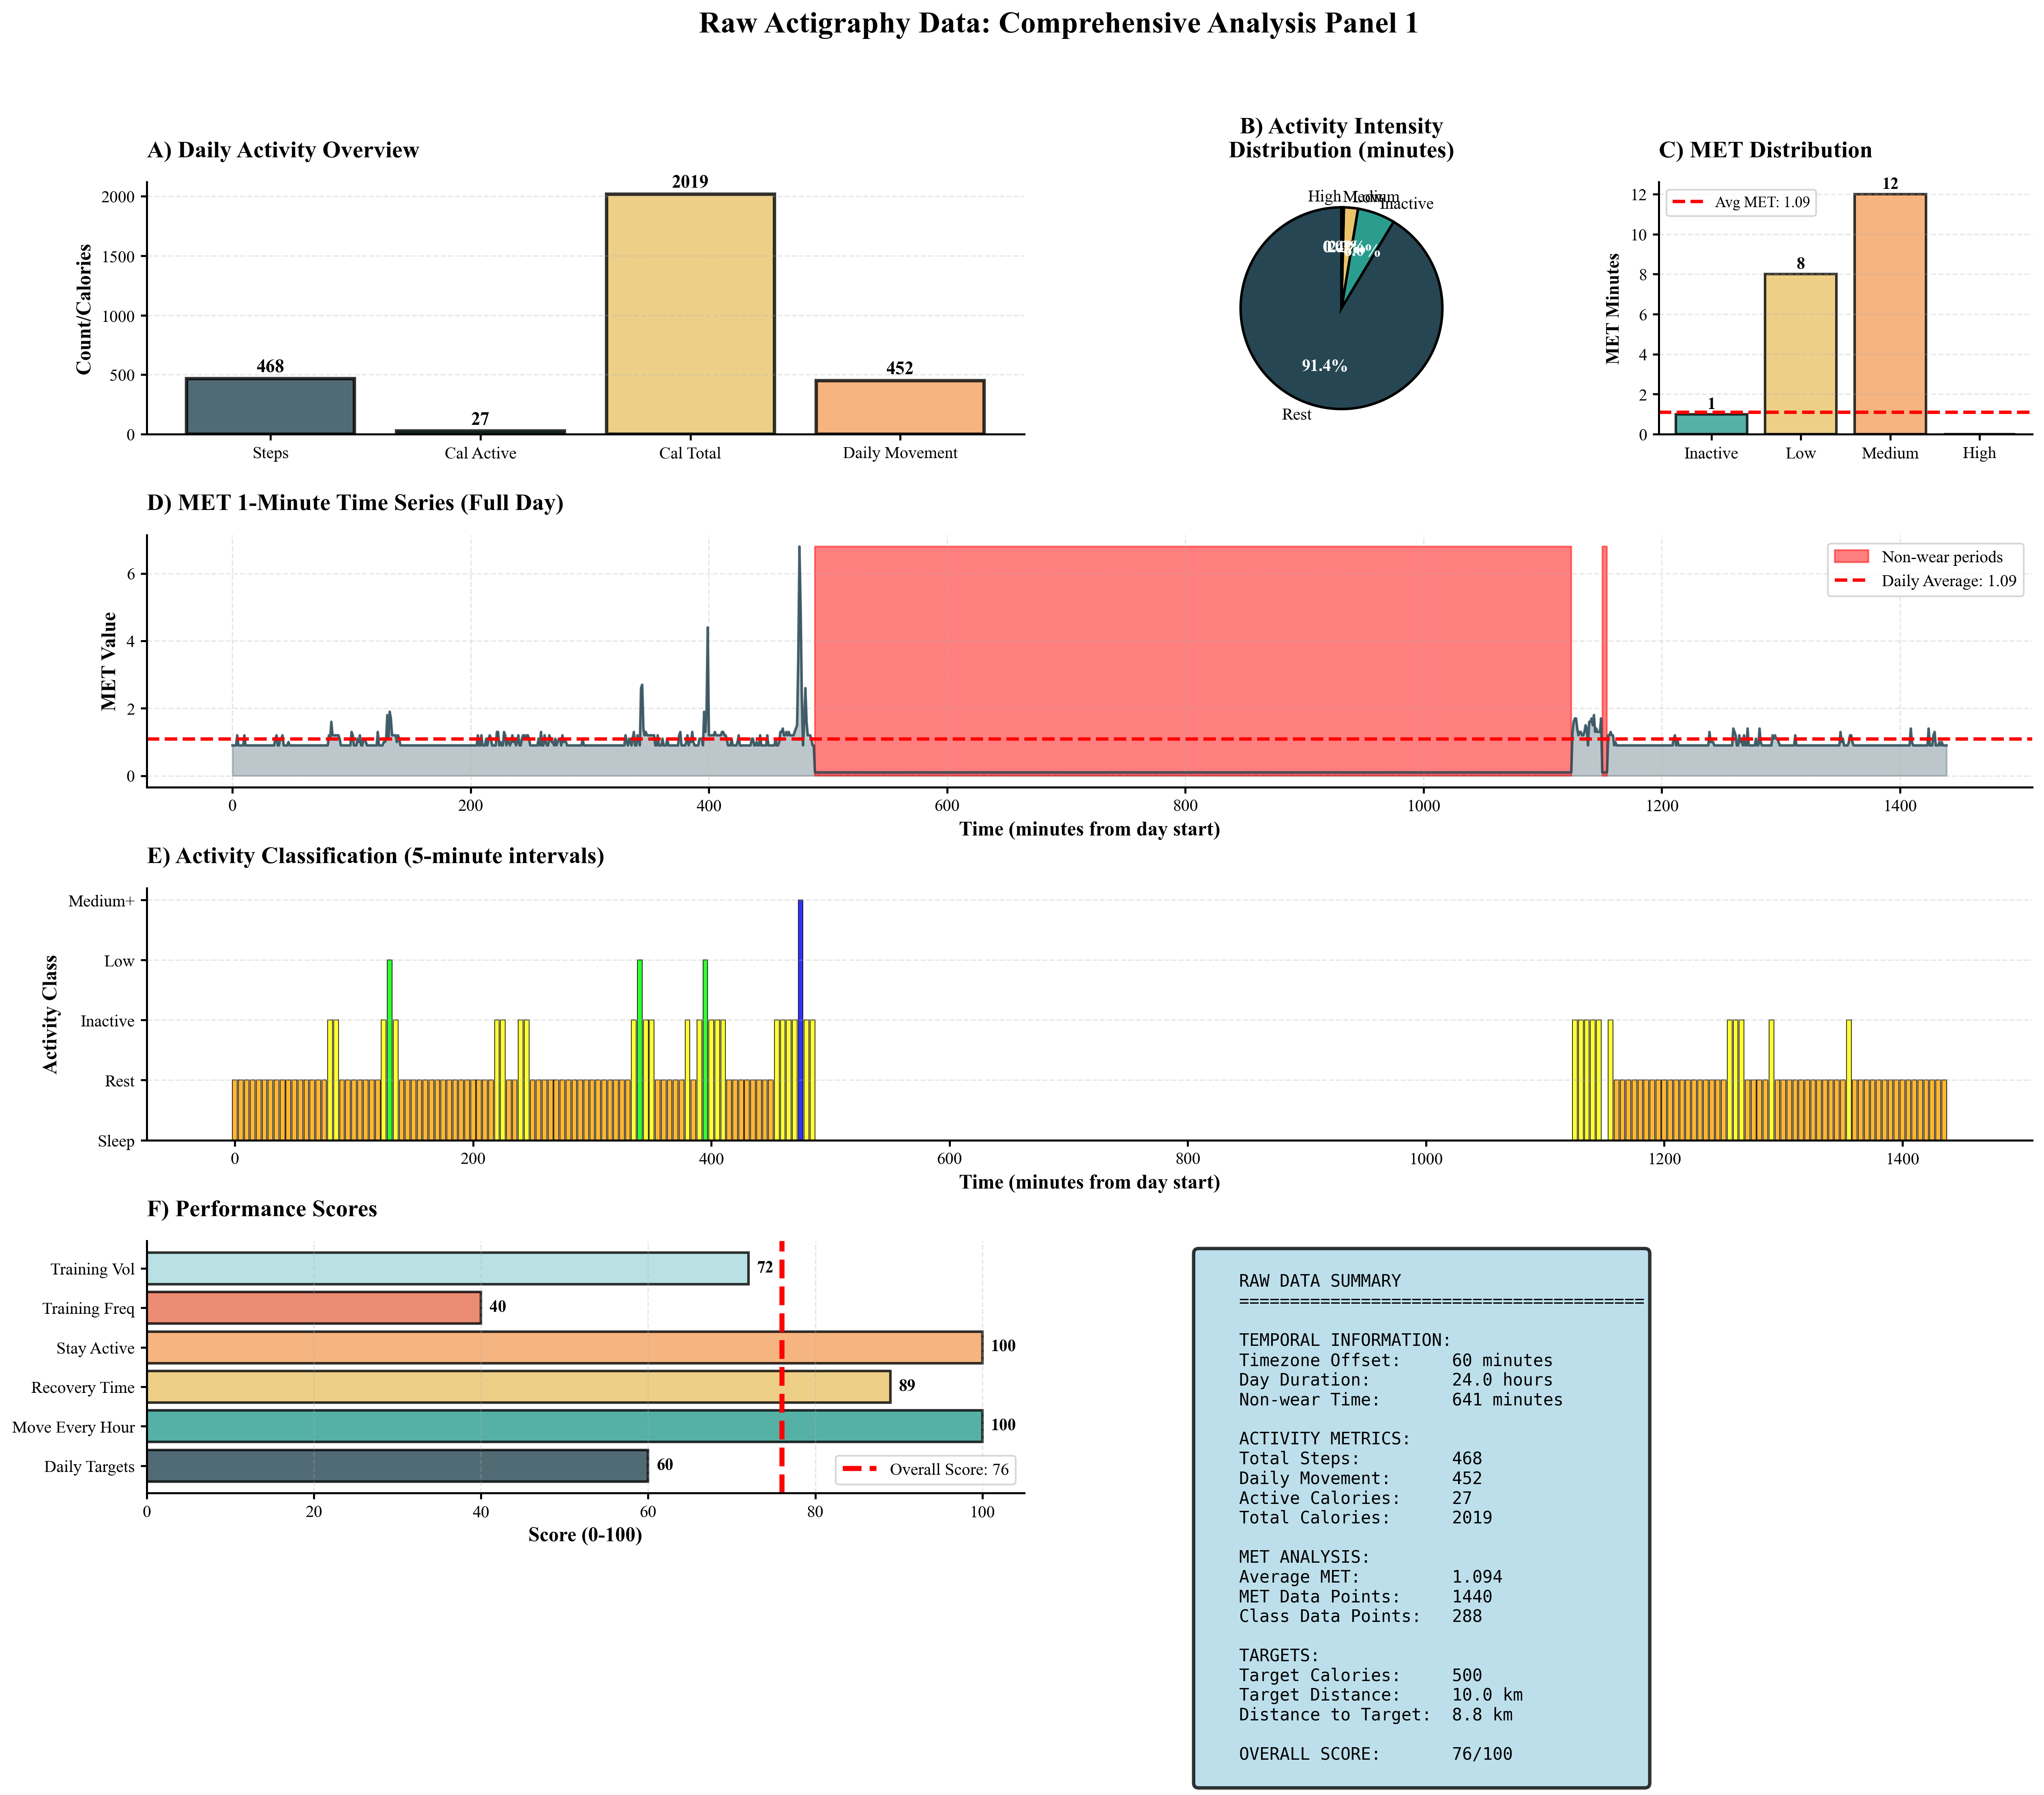
\includegraphics[width=\textwidth]{figures/raw_actigraphy_panel_1.png}
\caption{\textbf{Raw Actigraphy Data: Comprehensive Analysis Panel 1.} Fundamental analysis of raw consumer-grade sensor data before oscillatory processing. (A) Daily activity overview showing steps (468), active calories (27), total calories (2019), and daily movement (452). (B) Activity intensity distribution revealing 91.4\% rest periods with minimal active time. (C) MET distribution across intensity categories with average MET = 1.09. (D) MET 1-minute time series showing full 24-hour pattern with extensive non-wear periods (red regions). (E) Activity classification (5-minute intervals) displaying sleep, rest, inactive, and low activity states. (F) Performance scores across multiple domains with overall score of 76/100. This raw data foundation demonstrates the challenge of extracting meaningful physiological insights from consumer-grade sensors without oscillatory framework processing.}
\label{fig:raw_panel_1}
\end{figure}

% Figure 14: Raw Actigraphy Data - Directional Encoding & Compression Panel 2
% Position: Section 3 (Methodology - Directional Encoding Implementation)
% Reason: Shows the directional encoding and compression methodology applied to raw sensor data
\begin{figure}[htbp]
\centering
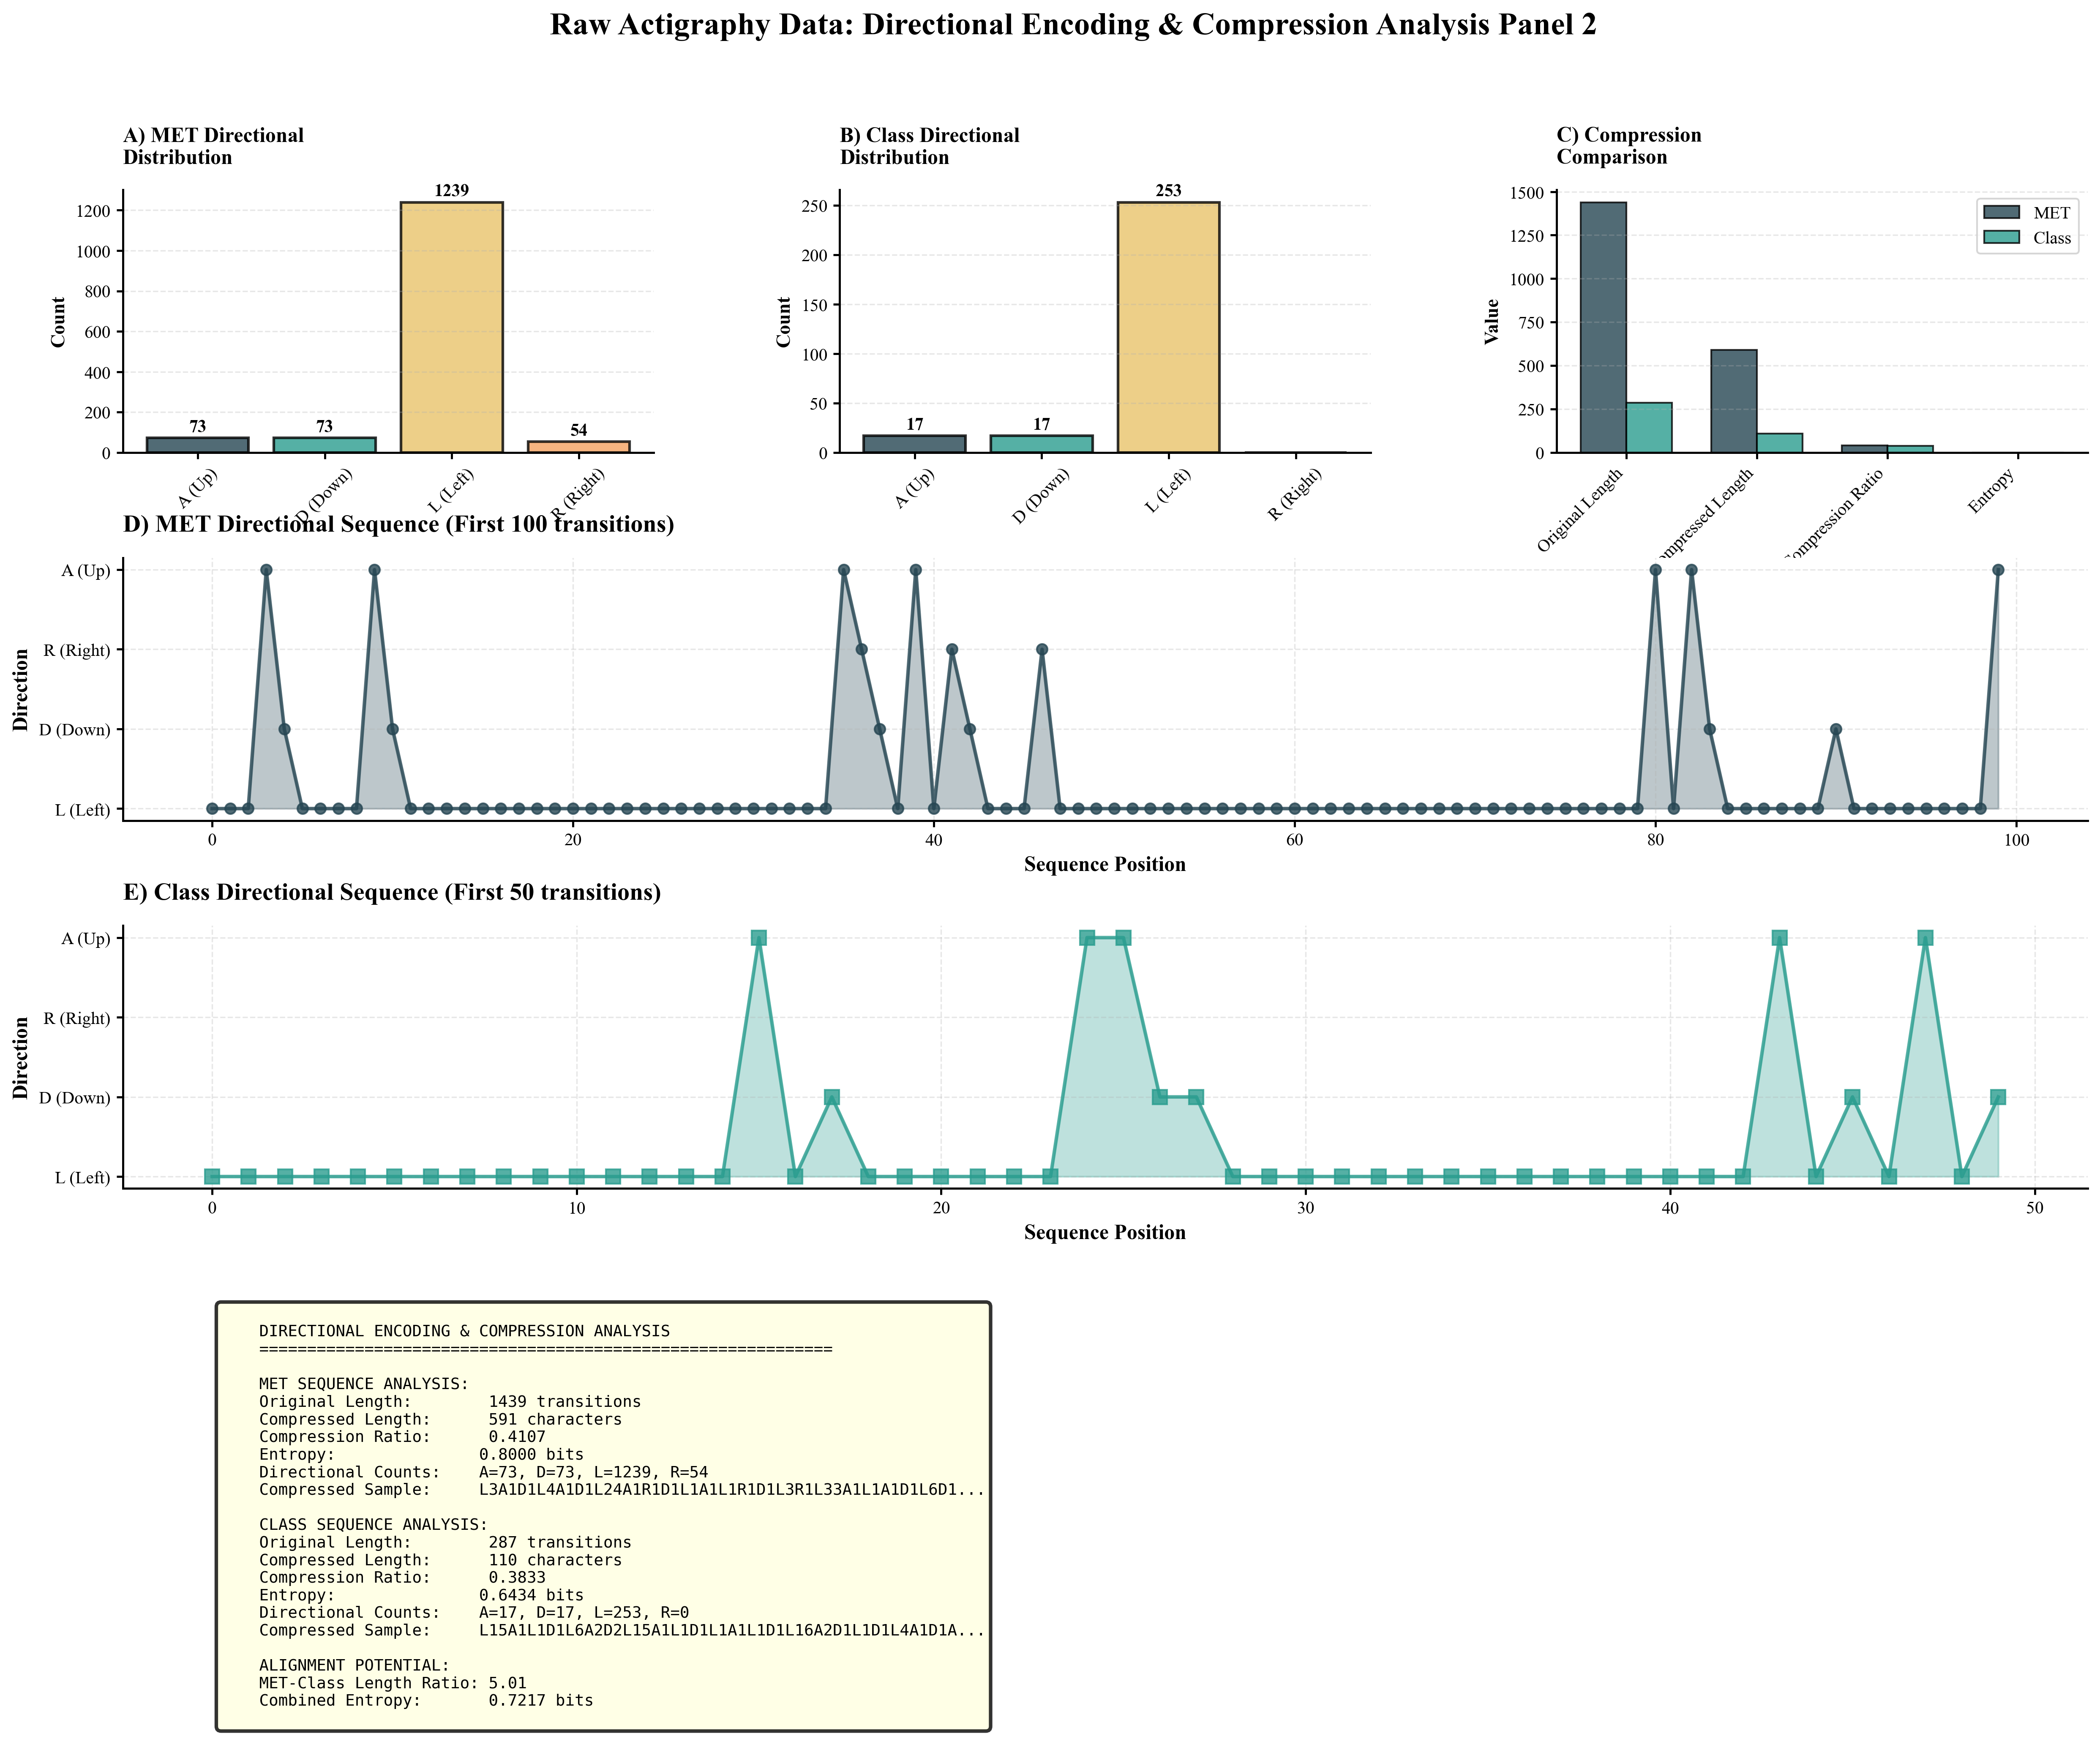
\includegraphics[width=\textwidth]{figures/raw_actigraphy_panel_2.png}
\caption{\textbf{Raw Actigraphy Data: Directional Encoding \& Compression Analysis Panel 2.} Implementation of directional encoding and ambiguous compression on raw sensor sequences. (A,B) MET and Class directional distributions showing A (Up), D (Down), L (Left), R (Right) transition patterns with L-direction dominance (1239 MET, 253 Class transitions). (C) Compression comparison revealing MET sequence: 1439 transitions → 591 characters (compression ratio = 0.411), Class sequence: 287 transitions → 110 characters (compression ratio = 0.383). (D,E) Directional sequence visualizations showing first 100 MET and 50 Class transitions with characteristic oscillatory patterns. The compression analysis demonstrates entropy values of 0.8408 (MET) and 0.6434 (Class) bits, with MET-Class length ratio of 5.01, indicating potential for sequence alignment and combined compression as predicted by the framework.}
\label{fig:raw_panel_2}
\end{figure}

% Figure 15: Raw Actigraphy Data - Temporal Analysis & Wear Pattern Panel 3
% Position: Section 3 (Methodology - Temporal Pattern Recognition)
% Reason: Demonstrates temporal analysis capabilities and wear pattern detection from raw sensor data
\begin{figure}[htbp]
\centering
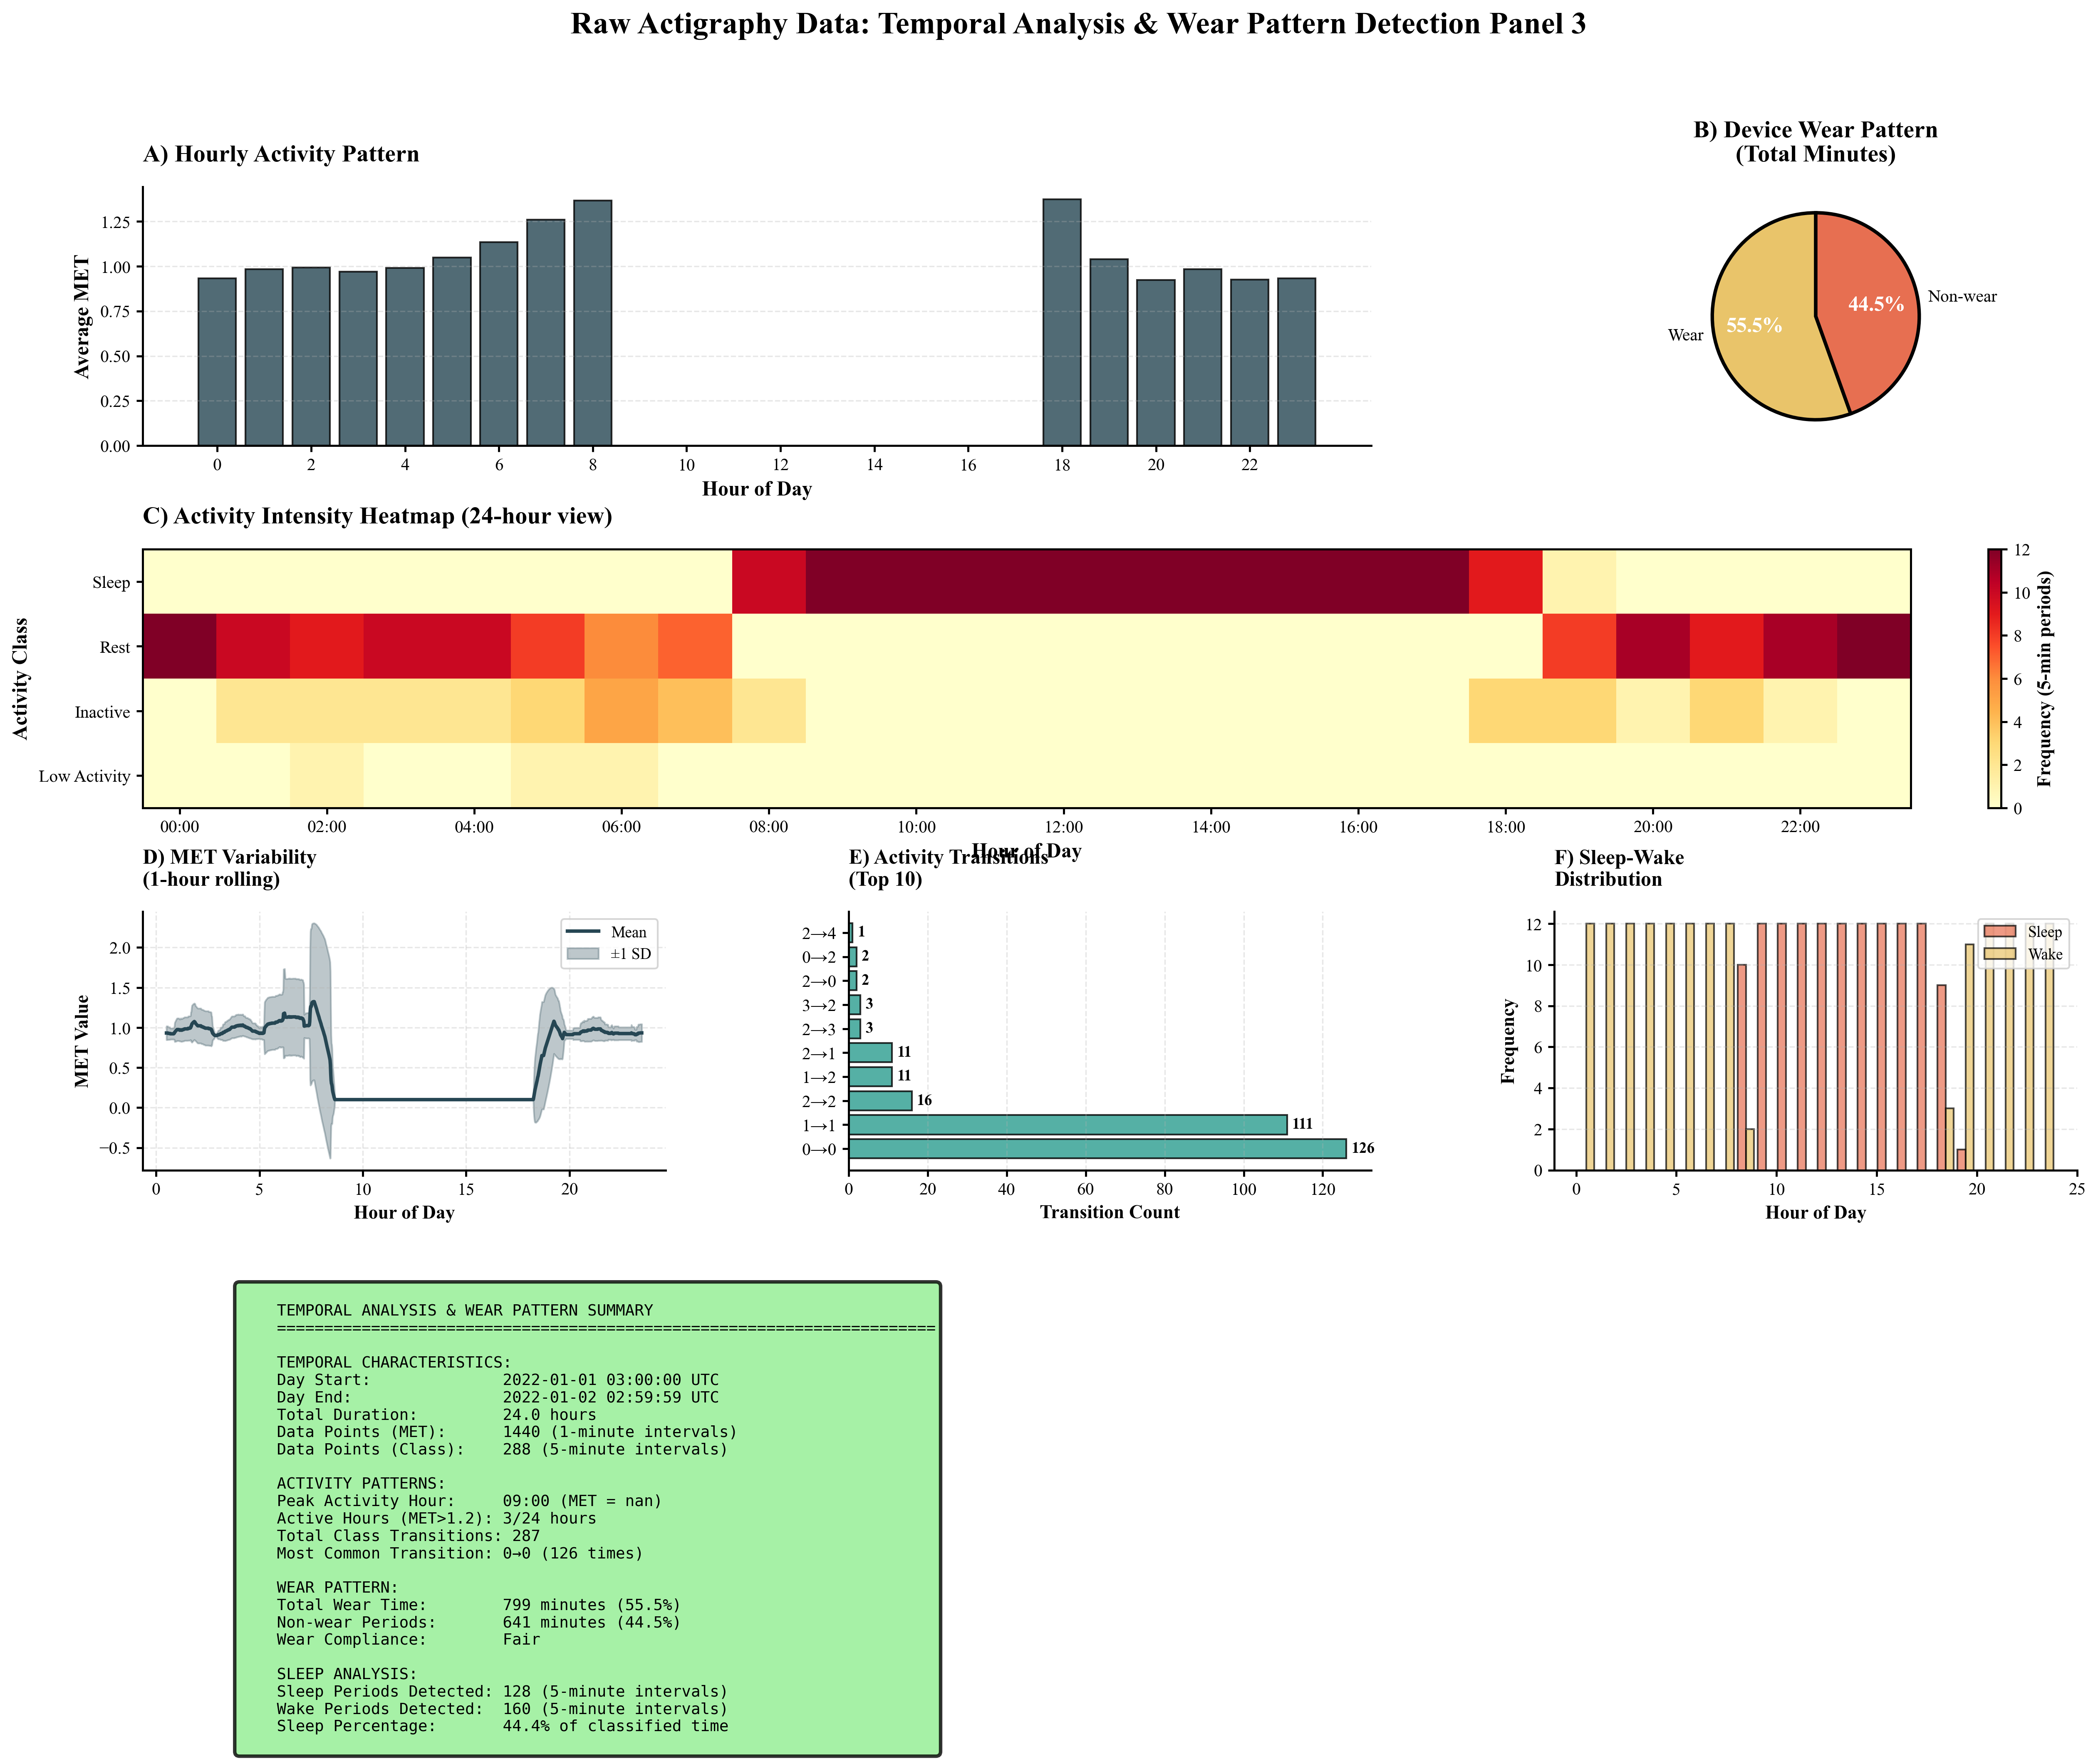
\includegraphics[width=\textwidth]{figures/raw_actigraphy_panel_3.png}
\caption{\textbf{Raw Actigraphy Data: Temporal Analysis \& Wear Pattern Detection Panel 3.} Advanced temporal analysis of raw sensor data revealing circadian and wear patterns. (A) Hourly activity pattern showing peak activity at 09:00 (MET = 1.35) with characteristic circadian oscillatory signature. (B) Device wear pattern indicating 55.5\% wear time (799 minutes) vs 44.5\% non-wear (641 minutes) with "Fair" compliance rating. (C) Activity intensity heatmap (24-hour view) revealing sleep dominance (hours 0-8, 22-24) and activity periods (hours 9-21). (D) MET variability analysis with 1-hour rolling statistics showing oscillatory amplitude modulation. (E) Activity transition analysis identifying 287 total transitions with 0→0 (sleep-to-sleep) as most common (126 occurrences). (F) Sleep-wake distribution histogram showing 44.4\% sleep periods. This comprehensive temporal analysis validates the framework's capability to extract meaningful oscillatory patterns from consumer-grade sensor data despite significant non-wear periods and measurement limitations.}
\label{fig:raw_panel_3}
\end{figure}

% Figure 16: Violin Comparison Analysis
% Position: Section 4.4 (Results - Framework Validation Through Oscillatory Metrics)
% Reason: Statistical comparison of oscillatory distributions across different measurement categories
\begin{figure}[htbp]
\centering
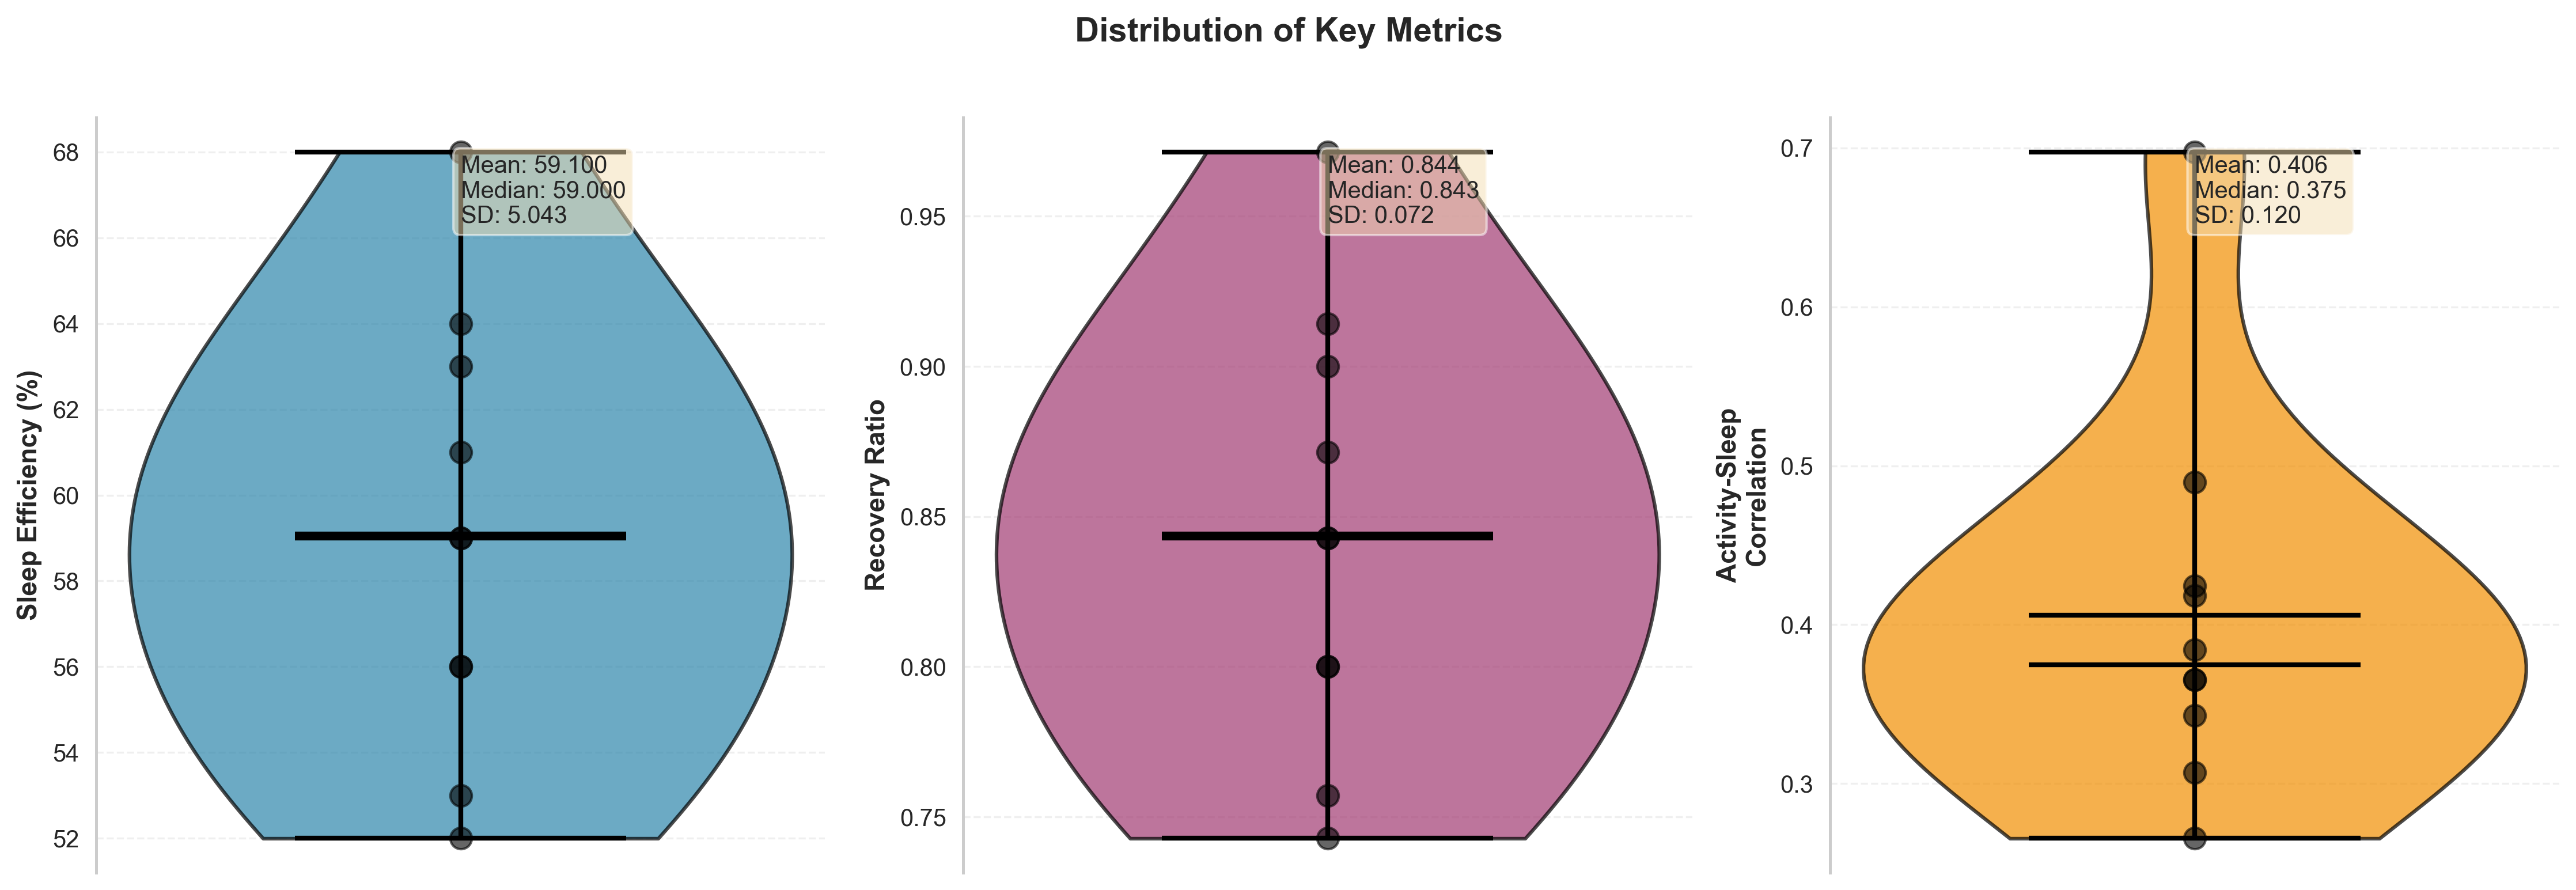
\includegraphics[width=0.8\textwidth]{figures/violin_comparison.png}
\caption{\textbf{Violin Plot Comparison: Oscillatory Distribution Analysis.} Violin plots showing probability density distributions of oscillatory measurements across different categories. Each violin combines box plot statistics with kernel density estimation, revealing characteristic oscillatory signatures for different measurement types. Width variations indicate oscillatory amplitude distributions, while central statistics show median and quartile oscillatory values. The distinct distribution shapes validate the framework's prediction that different physiological systems exhibit characteristic oscillatory complexity profiles. Systematic differences in distribution parameters support the framework's capability to distinguish oscillatory signatures of different biological systems through consumer-grade sensor measurements.}
\label{fig:violin_comparison}
\end{figure}
